%%%%%%%%%%%%%%%%%%%%%%%%%%%%%%%%%%%%%%%%%%%%%%%%%%%%%%%%%%%%%%%%%%%%%%%%%%%%%%%%
%% Plantilla de memoria en LaTeX para la EIF - Universidad Rey Juan Carlos
%%
%% Por Gregorio Robles <grex arroba gsyc.urjc.es>
%%     Grupo de Sistemas y Comunicaciones
%%     Escuela de Ingeniería de Fuenlabrada
%%     Universidad Rey Juan Carlos
%% (muchas ideas tomadas de Internet, colegas del GSyC, antiguos alumnos...
%%  etc. Muchas gracias a todos)
%%
%% La última versión de esta plantilla está siempre disponible en:
%%     https://github.com/gregoriorobles/plantilla-memoria
%%
%% Para obtener PDF, ejecuta en la shell:
%%   make
%% (las imágenes deben ir en PNG o JPG)

%%%%%%%%%%%%%%%%%%%%%%%%%%%%%%%%%%%%%%%%%%%%%%%%%%%%%%%%%%%%%%%%%%%%%%%%%%%%%%%%

\documentclass[a4paper, 12pt]{book}

%\usepackage[T1]{fontenc}
\usepackage{pgfgantt}
\usepackage[a4paper, left=2.5cm, right=2.5cm, top=3cm, bottom=3cm]{geometry}
\usepackage{times}
\usepackage[utf8]{inputenc}
\usepackage[spanish]{babel} % Comenta esta línea si tu memoria es en inglés
\usepackage{url}
%\usepackage[dvipdfm]{graphicx}
\usepackage{graphicx}
\usepackage{float}  %% H para posicionar figuras
\usepackage[nottoc, notlot, notlof, notindex]{tocbibind} %% Opciones de índice
\usepackage{latexsym}  %% Logo LaTeX
\usepackage{listings}
\usepackage{xcolor}
\usepackage{tabularx}
\usepackage{array}
\usepackage{booktabs}
\usepackage{hyperref}

\lstset{
  basicstyle=\ttfamily\footnotesize,
  breaklines=true,
  backgroundcolor=\color{gray!10},
  frame=single,
  captionpos=b
}


% Escribe el título y el nombre del autor / autora para que se use bien
% en otras partes de la plantilla
% Dependiendo de las partes de la plantilla, a veces aparecerán tal
% cual los escribas, a veces totalmente en mayúsculas, a veces de otras
% formas
\title{Edición de Escenas 3D mediante Voz}
\author{Pablo Esteban Camuendo Carlosama}

% Guarda el título, el autor y la fecha en variables
\makeatletter
\let\thetitle\@title
\let\theauthor\@author
\let\thedate\@date
\let\cleardoublepage\clearpage
\makeatother

\renewcommand{\baselinestretch}{1.5}  %% Interlineado

\begin{document}

\renewcommand{\refname}{Bibliografía}  %% Renombrando
\renewcommand{\appendixname}{Apéndice}


%%%%%%%%%%%%%%%%%%%%%%%%%%%%%%%%%%%%%%%%%%%%%%%%%%%%%%%%%%%%%%%%%%%%%%%%%%%%%%%%
% PORTADA

\begin{titlepage}
\begin{center}

\includegraphics[scale=0.6]{img/URJ_logo_Color_POS.png}

\vspace{1.75cm}

\LARGE
ESCUELA DE INGENIERÍA DE FUENLABRADA
\vspace{1cm}

\LARGE
INGENIERÍA EN SISTEMAS AUDIOVISUALES Y MULTIMEDIA

\vspace{1cm}
\LARGE
\textbf{TRABAJO FIN DE GRADO/MÁSTER}

\vspace{2cm}

\Large
\MakeUppercase{\thetitle}

\vspace{2cm}

\large
Autor : \theauthor \\
Tutor : Dr. Jesús María González Barahona\\
Cotutor: (si procede)
\vspace{1cm}

\large
Curso académico 2024/2025

\end{center}
\end{titlepage}

\newpage
\mbox{}
\thispagestyle{empty} % para que no se numere esta pagina



%%%%%%%%%%%%%%%%%%%%%%%%%%%%%%%%%%%%%%%%%%%%%%%%%%%%%%%%%%%%%%%%%%%%%%%%%%%%%%%%
%%%% Licencia
\clearpage
\pagenumbering{gobble}
\chapter*{}

\vspace{12cm}

%% Licencia de publicación en abierto elegida
%% Ver detalles en https://ofilibre.urjc.es/guias/tfg-abierto/

\begin{flushright}
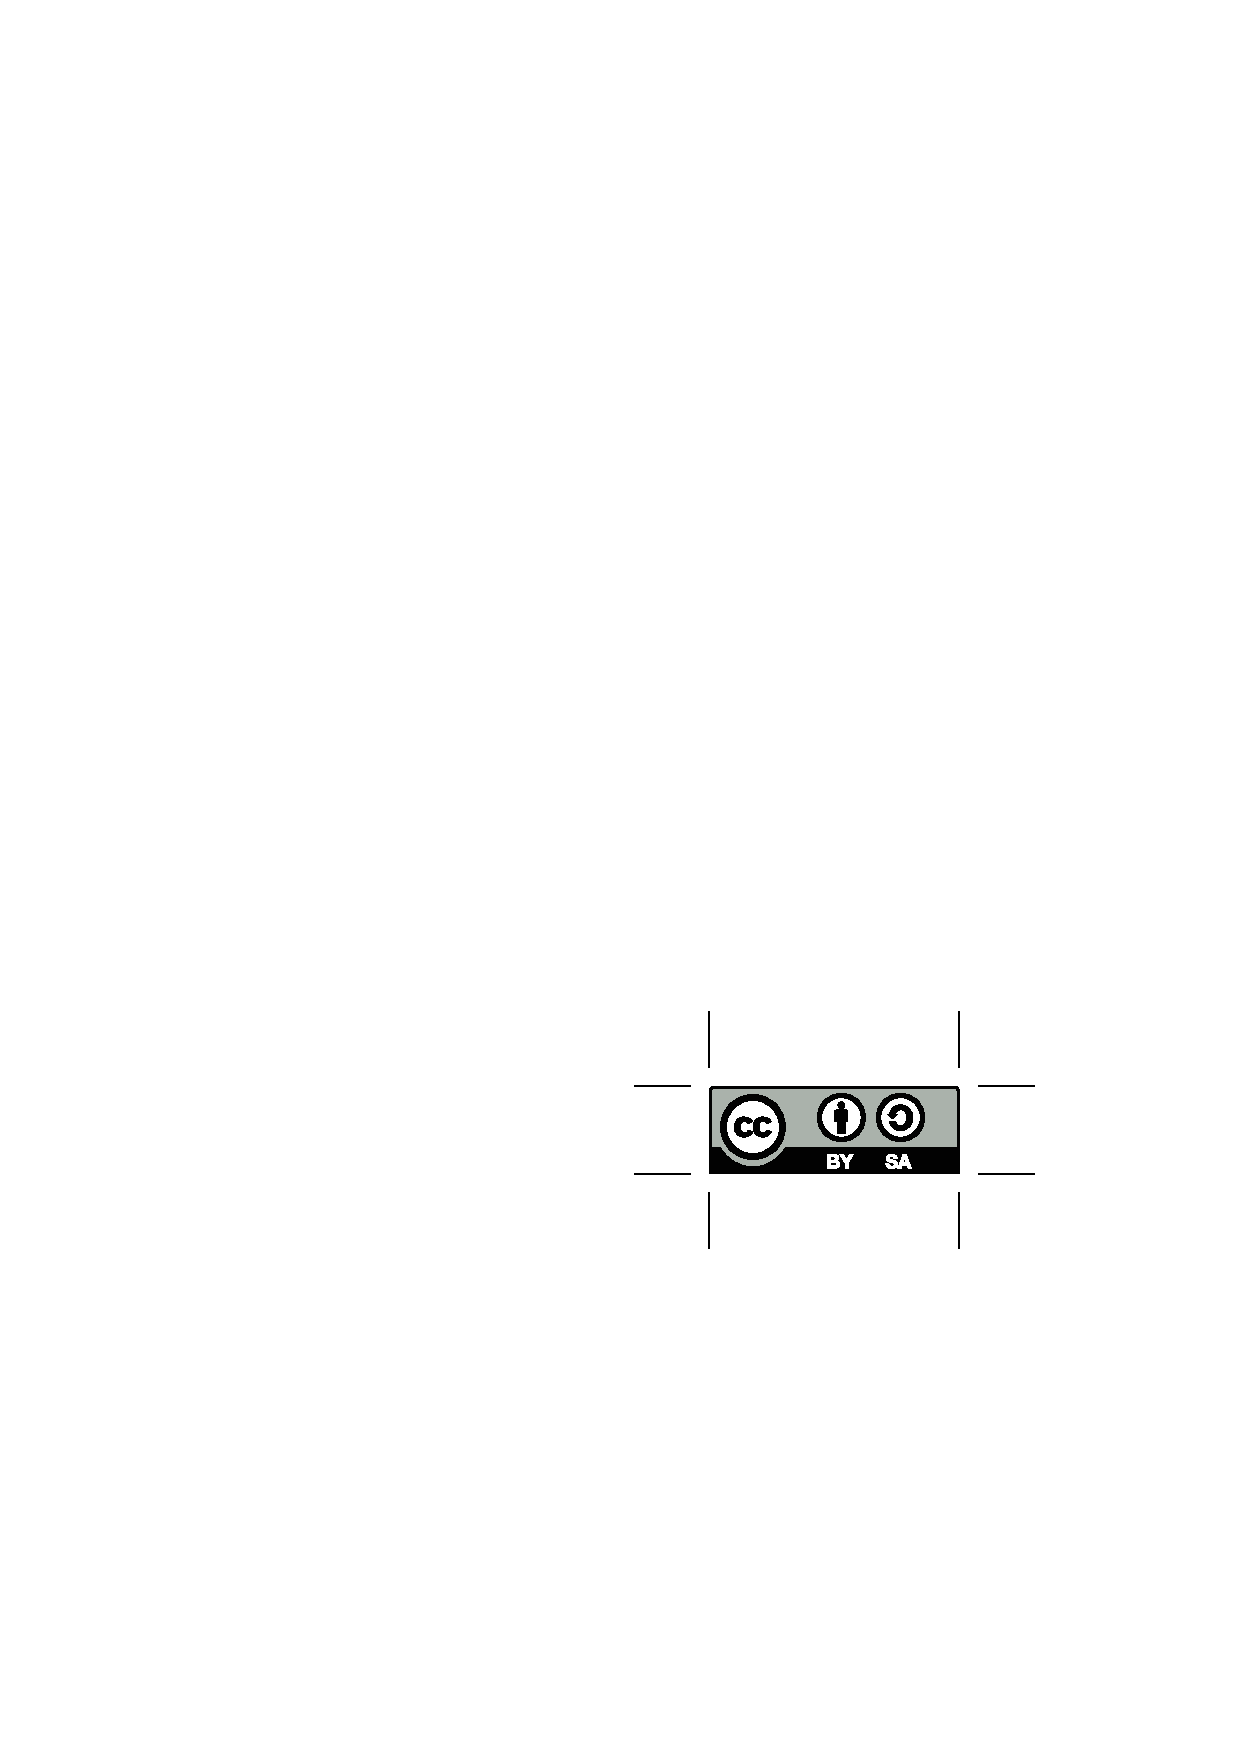
\includegraphics[scale=0.6]{img/by-sa}
%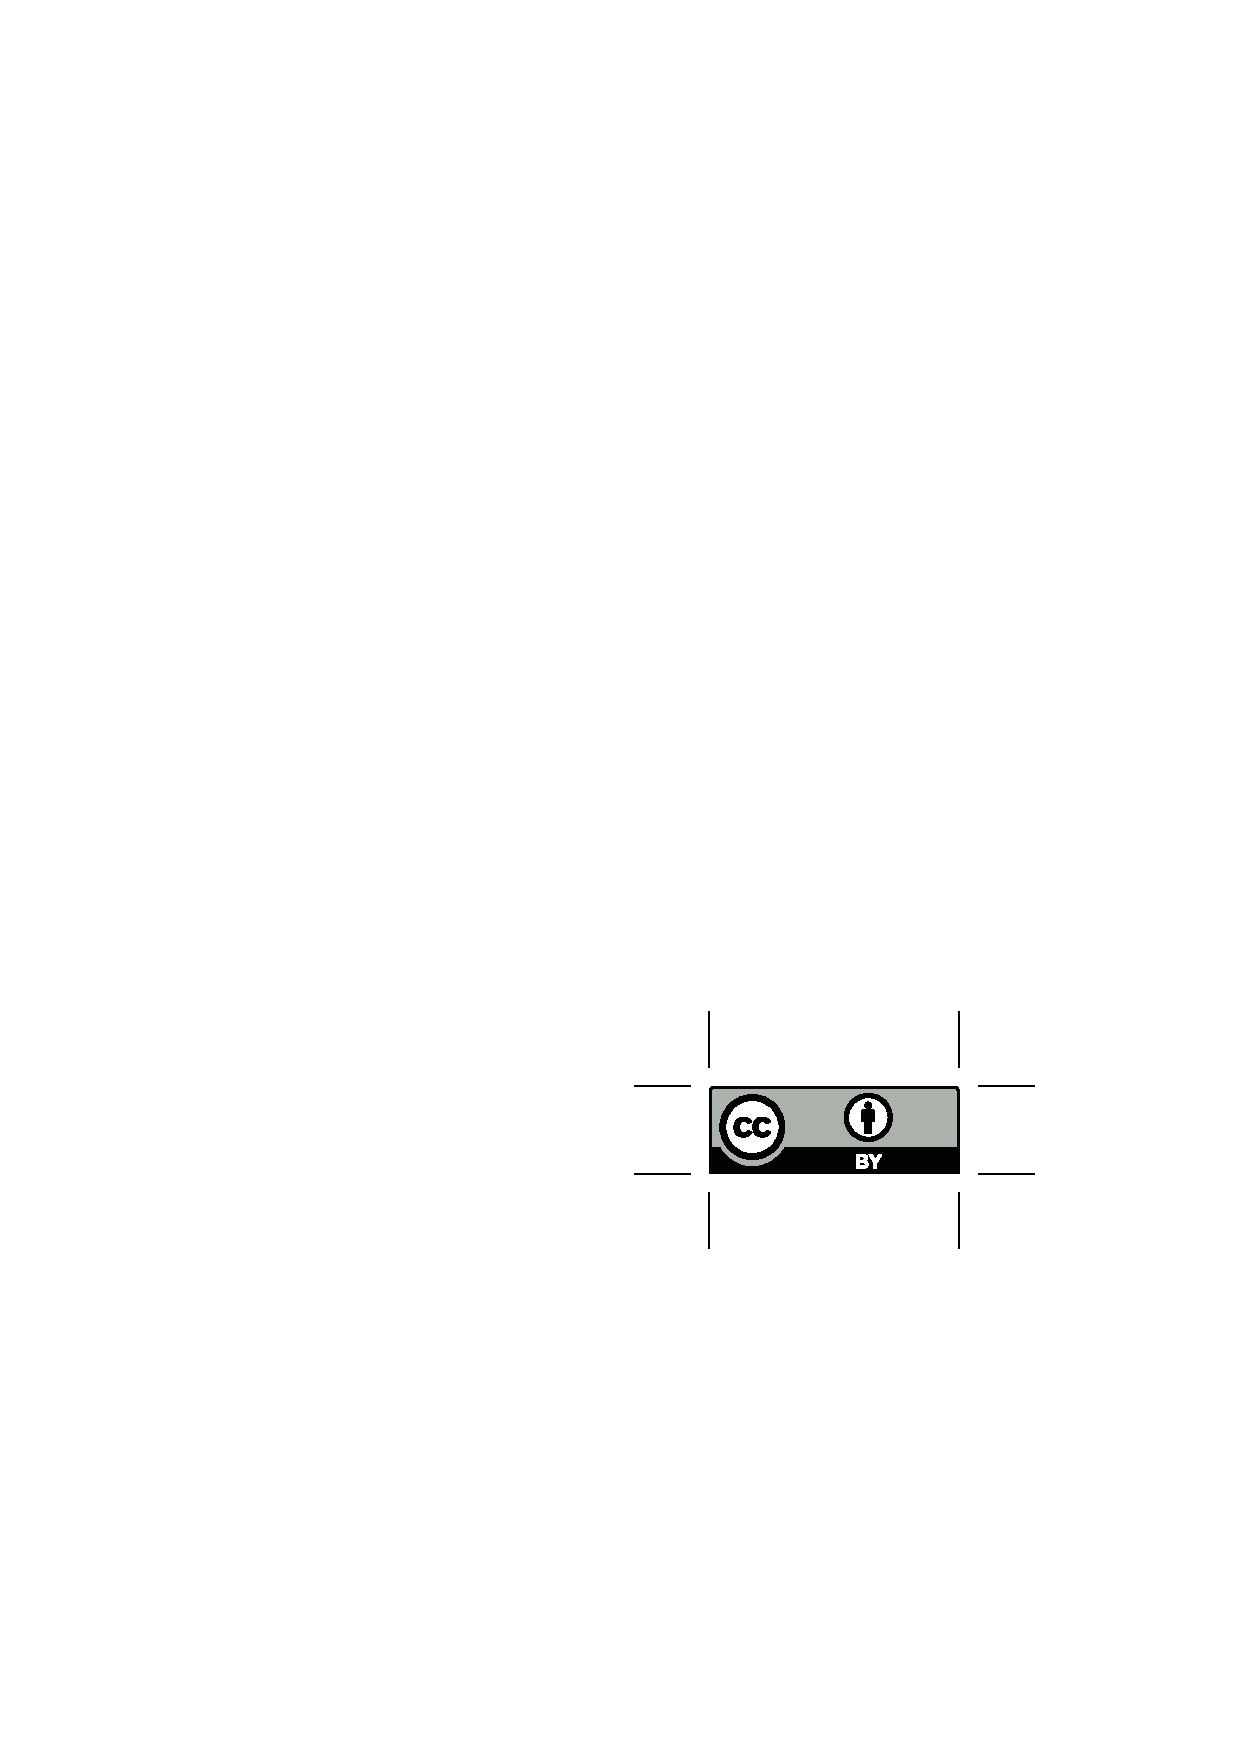
\includegraphics[scale=0.6]{img/by}

%% Poner el año adecuado
\noindent©2025 \theauthor  \\
Algunos derechos reservados  \\
Este documento se distribuye bajo la licencia \\
``Atribución-CompartirIgual 4.0 Internacional'' de Creative Commons, \\
disponible en \\
\url{https://creativecommons.org/licenses/by-sa/4.0/deed.es}
\end{flushright}

%%%%%%%%%%%%%%%%%%%%%%%%%%%%%%%%%%%%%%%%%%%%%%%%%%%%%%%%%%%%%%%%%%%%%%%%%%%%%%%%
%%%% Dedicatoria

\chapter*{}
\pagenumbering{Roman} % para comenzar la numeracion de paginas en numeros romanos
\begin{flushright}
\textit{Dedicado a \\
mi familia.}
\end{flushright}

%%%%%%%%%%%%%%%%%%%%%%%%%%%%%%%%%%%%%%%%%%%%%%%%%%%%%%%%%%%%%%%%%%%%%%%%%%%%%%%%
%%%% Agradecimientos

\chapter*{Agradecimientos}
%\addcontentsline{toc}{chapter}{Agradecimientos} % si queremos que aparezca en el índice
\markboth{AGRADECIMIENTOS}{AGRADECIMIENTOS} % encabezado 

Quisiera expresar mi más sincero agradecimiento a todas las personas e instituciones que han hecho posible la realización de esta tesis de grado.

En primer lugar, mi familia, durante todos estos años de estudio, por su apoyo incondicional y esfuerzo, su comprensión y aliento continuo. Su fe en mí es la mayor inspiración. Ellos siempre han dicho que la educación es la base de todo lo que puedo construir a continuación y es gracias a ellos que he podido llegar aquí. Gracias, mamá y papá

A mi hermana, que ha sido un constante apoyo y de la cual quiero ser un ejemplo a seguir, que sepa que el desarrollo de uno mismo es difícil, pero satisfactorio al final.

A mi tutor de tesis, por su guía, paciencia y conocimientos compartidos a lo largo de este proceso. Su experiencia ha sido crucial para el desarrollo de este trabajo.

Finalmente, a todos aquellos que de una u otra manera han contribuido a mi crecimiento personal y profesional durante mi etapa universitaria.

A todos, mi más profunda gratitud.


%%%%%%%%%%%%%%%%%%%%%%%%%%%%%%%%%%%%%%%%%%%%%%%%%%%%%%%%%%%%%%%%%%%%%%%%%%%%%%%%
%%%% Resumen

\chapter*{Resumen}
%\addcontentsline{toc}{chapter}{Resumen} % si queremos que aparezca en el índice
\markboth{RESUMEN}{RESUMEN} % encabezado

RESUMEN LO HAGO AL FINAL \dots



%%%%%%%%%%%%%%%%%%%%%%%%%%%%%%%%%%%%%%%%%%%%%%%%%%%%%%%%%%%%%%%%%%%%%%%%%%%%%%%%
%%%% Resumen en inglés

\chapter*{Summary}
%\addcontentsline{toc}{chapter}{Summary} % si queremos que aparezca en el índice
\markboth{SUMMARY}{SUMMARY} % encabezado

Here comes a translation of the ``Resumen'' into English. 
Please, double check it for correct grammar and spelling.
As it is the translation of the ``Resumen'', which is supposed to be written at the end, this as well should be filled out just before submitting.


%%%%%%%%%%%%%%%%%%%%%%%%%%%%%%%%%%%%%%%%%%%%%%%%%%%%%%%%%%%%%%%%%%%%%%%%%%%%%%%%
%%%%%%%%%%%%%%%%%%%%%%%%%%%%%%%%%%%%%%%%%%%%%%%%%%%%%%%%%%%%%%%%%%%%%%%%%%%%%%%%
% ÍNDICES %
%%%%%%%%%%%%%%%%%%%%%%%%%%%%%%%%%%%%%%%%%%%%%%%%%%%%%%%%%%%%%%%%%%%%%%%%%%%%%%%%

% Las buenas noticias es que los índices se generan automáticamente.
% Lo único que tienes que hacer es elegir cuáles quieren que se generen,
% y comentar/descomentar esa instrucción de LaTeX.

%%%% Índice de contenidos
\tableofcontents 
%%%% Índice de figuras
\cleardoublepage
%\addcontentsline{toc}{chapter}{Lista de figuras} % para que aparezca en el indice de contenidos
\listoffigures % indice de figuras
%%%% Índice de tablas
%\cleardoublepage
%\addcontentsline{toc}{chapter}{Lista de tablas} % para que aparezca en el indice de contenidos
%\listoftables % indice de tablas


%%%%%%%%%%%%%%%%%%%%%%%%%%%%%%%%%%%%%%%%%%%%%%%%%%%%%%%%%%%%%%%%%%%%%%%%%%%%%%%%
%%%%%%%%%%%%%%%%%%%%%%%%%%%%%%%%%%%%%%%%%%%%%%%%%%%%%%%%%%%%%%%%%%%%%%%%%%%%%%%%
% INTRODUCCIÓN %
%%%%%%%%%%%%%%%%%%%%%%%%%%%%%%%%%%%%%%%%%%%%%%%%%%%%%%%%%%%%%%%%%%%%%%%%%%%%%%%%

\cleardoublepage
\chapter{Introducción}
\label{sec:intro} % etiqueta para poder referenciar luego en el texto con ~\ref{sec:intro}
\pagenumbering{arabic} % para empezar la numeración de página con números
Con el gran avance en tecnologías, la realidad virtual (VR) ha experimentado un gran crecimiento en los últimos años, gracias a la evolución de tecnologías web accesibles y de código abierto. 
A-Frame es un framework potente y versátil, basado en WebXR y Three.js, que facilita la creación y configuración de escenas aprovechando directamente el navegador usando HTML y JavaScript.

Unido a este framework tendremos el desarrollo del reconocimiento del habla que permitirá controlar la escena mediante comandos de voz.
La sinergia entre A-Frame y el control por voz representa un enfoque innovador con el potencial de transformar la accesibilidad, la usabilidad y la inmersión en las experiencias de realidad virtual, ofreciendo una alternativa intuitiva a los métodos de interacción tradicionales.

Este proyecto surge de la inquietud por investigar nuevas formas de interacción en entornos 3D web. 
A día de hoy existen avances significativos en la creación visual de escenas virtuales, 
la edición y manipulación de objetos puede resultar en ocasiones compleja y poco intuitiva. 
La idea de un editor controlado por voz sería como una alternativa prometedora para agilizar el flujo de trabajo y mejorar la accesibilidad para usuarios con diferentes necesidades.

Actualmente, se ha avanzado en la exploración de diferentes arquitecturas y sistemas de componentes para la implementación de un editor 3D dirigido por voz. Como resultado de esta investigación, se ha desarrollado un prototipo funcional que permite la creación y edición básica de objetos en una escena 3D mediante comandos de voz. Sin embargo, es importante señalar que la aplicación aún se encuentra en una fase de desarrollo y no está completamente pulida. El trabajo futuro se centrará en refinar la funcionalidad existente, ampliar el conjunto de comandos de voz y mejorar la estabilidad y el rendimiento general del sistema.

\section{Estructura de la memoria}
\label{sec:estructura}

El resto de la memoria se estructurara de la siguiente manera:

\begin{itemize}
    \item ~\ref{chap:Tecnologías utilizadas} Tecnologías utilizadas: Se muestran todas las tecnologías utilizadas durante el desarrollo del proyecto, desde las principales como A-Frame para la construcción de entornos inmersivos en el navegador, hasta herramientas auxiliares como Node.js o WebXR. Se da una breve descripción de cada tecnología, el contexto de uso y su papel dentro de cada una de las demos.
  
    \item ~\ref{chap:Desarollo} Desarrollo del Proyecto: Se detalla el proceso completo de creación, donde se implementaron dos versiones de la demo: una que usa la Web Speech API directamente en el navegador, y otra que envía audio a un servidor local para procesarlo con Assembly AI.
  
    \item ~\ref{chap:resultados}  Resultados:
 Aquí se muestra el resultado final de ambas demos
\begin{itemize}
  \item Descripción para el usuario: Se explica qué funcionalidades incluye cada demo, cómo se activan los comandos por voz y cómo se muestra la transcripción dentro del entorno 3D. 
  \item Descripción del comportamiento de la interfaz: Se detalla cómo se representa la transcripción en la escena VR/AR, así como la lógica de actualización dinámica de objetos en el espacio virtual.
\end{itemize}
    \item ~\ref{chap:experimentos} Experimentos y validación  
    \item ~\ref{chap:conclusiones} Conclusiones 
\end{itemize}

%%%%%%%%%%%%%%%%%%%%%%%%%%%%%%%%%%%%%%%%%%%%%%%%%%%%%%%%%%%%%%%%%%%%%%%%%%%%%%%%
% OBJETIVOS %
%%%%%%%%%%%%%%%%%%%%%%%%%%%%%%%%%%%%%%%%%%%%%%%%%%%%%%%%%%%%%%%%%%%%%%%%%%%%%%%%
\section{Objetivo general} % título de sección (se muestra)
\label{sec:objetivo-general} % identificador de sección (no se muestra, es para poder referenciarla)

El trabajo de fin de grado consiste en explorar diversas metodologías para la implementación de un editor 3D dirigido por voz, 
finalizando en el desarrollo de un prototipo funcional basado en un sistema de componentes que demuestre la viabilidad de la creación y edición de escenas 3D mediante comandos de voz en navegadores web compatibles.
En entornos de escritorio o dispositivos VR/AR como las gafas Quest3

\section{Objetivos específicos}
\label{sec:objetivos-especificos}

\begin{itemize}
\item Explorar distintas soluciones para encontrar una que funcione bien en gafas tipo Quest3 y otra en el navegador de escritorio.
\item Explorar qué opciones se tienen para Speech-to-text en un entorno como un navegador o dispositivos tipo Quest3.
\item Conseguir transcripciones del usuario con la aplicación.
\item Reconocimiento de órdenes concretas para interactuar con el editor de escenas.
\item Explorar distintas soluciones para encontrar una que funcione bien en gafas tipo Quest3 y otra en el navegador de escritorio.
\item Hacer que el prototipo soporte comandos como crear, editar, mover\dots
\item Construir el prototipo de forma que funcione en el navegador en escritorio y en equipos VR/AR como las gafas Quest3.
\item Utilizar para la construcción el framework A-Frame, porque se adapta especialmente bien al objetivo anterior. 
\item Realización de un prototipo modular.
\end{itemize}

%%%%%%%%%%%%%%%%%%%%%%%%%%%%%%%%%%%%%%%%%%%%%%%%%%%%%%%%%%%%%%%%%%%%%%%%%%%%%%%%
%%%%%%%%%%%%%%%%%%%%%%%%%%%%%%%%%%%%%%%%%%%%%%%%%%%%%%%%%%%%%%%%%%%%%%%%%%%%%%%%
% ESTADO DEL ARTE %
%%%%%%%%%%%%%%%%%%%%%%%%%%%%%%%%%%%%%%%%%%%%%%%%%%%%%%%%%%%%%%%%%%%%%%%%%%%%%%%%

\cleardoublepage
\cleardoublepage % empezamos en página impar

\chapter{Tecnologías utilizadas}
\label{chap:Tecnologías utilizadas}

El proyecto utiliza la interfaz webkitSpeechRecognition para implementar el reconocimiento de voz en el navegador. Esta interfaz es una versión específica para WebKit de la API de reconocimiento de voz de la Web Speech API, que permite a las aplicaciones web convertir el habla en texto.

Además, el proyecto emplea tecnologías web estándar como HTML, CSS y JavaScript para construir la interfaz de usuario y manejar la lógica del cliente. Estas tecnologías trabajan conjuntamente para proporcionar una experiencia interactiva de reconocimiento de voz directamente en el navegador.

Se creó un flujo de trabajo extra para el uso del proyecto en gafas de VR/AR, debido a la creación de un servidor privado lanzado con Node.js → para ejecutar el servidor back-end. framework HTTP → Para manejar las solicitudes del cliente. Assembly AI API → Servicio externo de reconocimiento de voz. Fetch → Para enviar los datos de audio a Assembly AI desde el servidor.

** PONER ALGUNA CITA EN CADA APARTADO
SPEECH 
** W3C
CONSTRUCCIÓN SOBRE LOS OBJETOS
A-FRAME > THREE > WEBXR > WEBGL
A FRAME HABLAR DE COMPONENTES, CAPTURAS, ACCIONES, LLAMADOS, CÓDIGO, ESCENA


\section{Tecnologias de reconocimiento de voz} 
\label{sec:seccion1}

El reconocimiento de voz en navegadores permite a los usuarios interactuar con aplicaciones web y contenido utilizando su voz en lugar de escribir. Esto abre un mundo  de posibilidades para la accesibilidad, la productividad y la creación de experiencias de usuario más interactivas.

\subsection{Whisper}

En primera instancia se planeaba trabajar con Whisper, un modelo de 'Speech Recognition' de OpenAI que se destaca por su capacidad para transcribir audio en múltiples idiomas con alta precisión, incluso en condiciones de ruido o con variaciones en el acento del hablante, con el objetivo de integrarlo al proyecto.

Whisper\footnote{Whisper OpenAI github ~\cite{whisper}.} jugaba una parte esencial. Se eligió debido a la arquitectura robusta y de código libre. Como parte de la investigación, se analizaron los requisitos técnicos para la implementación, incluyendo dependencias, consumo de recursos, y compatibilidad con otros componentes del sistema.

\begin{figure}[H]
    \centering
    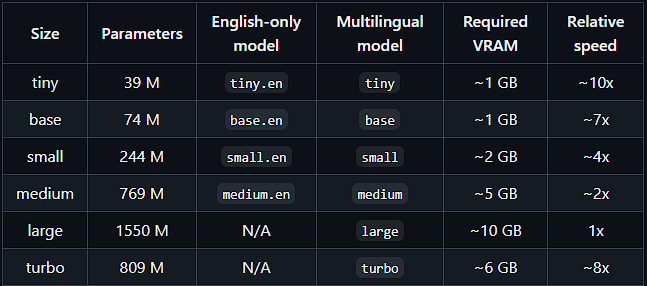
\includegraphics[width=0.8\linewidth]{img/Whisper_github.png}
    \caption{Modelos de Whisper}
    \label{fig:models-Whisper}
\end{figure}

Whisper presenta los modelos que se pueden ver en la Figura~\ref{fig:models-Whisper}. Se pueden observar diferentes tamaños de modelos, cada uno con distintos niveles de precisión, velocidad y requerimientos de hardware.

Los modelos más grandes (medium,large)son altamente demandantes de GPU, esto hace que los modelos tengan mucha más precisión, pero que su velocidad sea más afectada. Para una menor latencia, los modelos más pequeños (tiny, base, small) son mejores, ya que su demanda de hardware es menor.

Alguno de los problemas que presentó Whisper fue el tamaño de los modelos, ya que incluso el modelo más pequeño (tiny) pesa varios cientos de MB. Se necesita PyTorch y dependencias que no están disponibles en entornos web estándar (como JS/WebAssembly). Además del uso intensivo de GPU/CPU, lo cual no es viable en la mayoría de navegadores móviles o de escritorio.

\subsection{Whisper Web}

Actualmente, algunos proyectos han empezado a portar versiones ligeras al navegador (construcciones en WebAssembly u ONNX). Un ejemplo de esto es Whisper Web\footnote{Whisper Web Hugging Face ~\cite{whisperweb}.}

\begin{figure}[H]
    \centering
    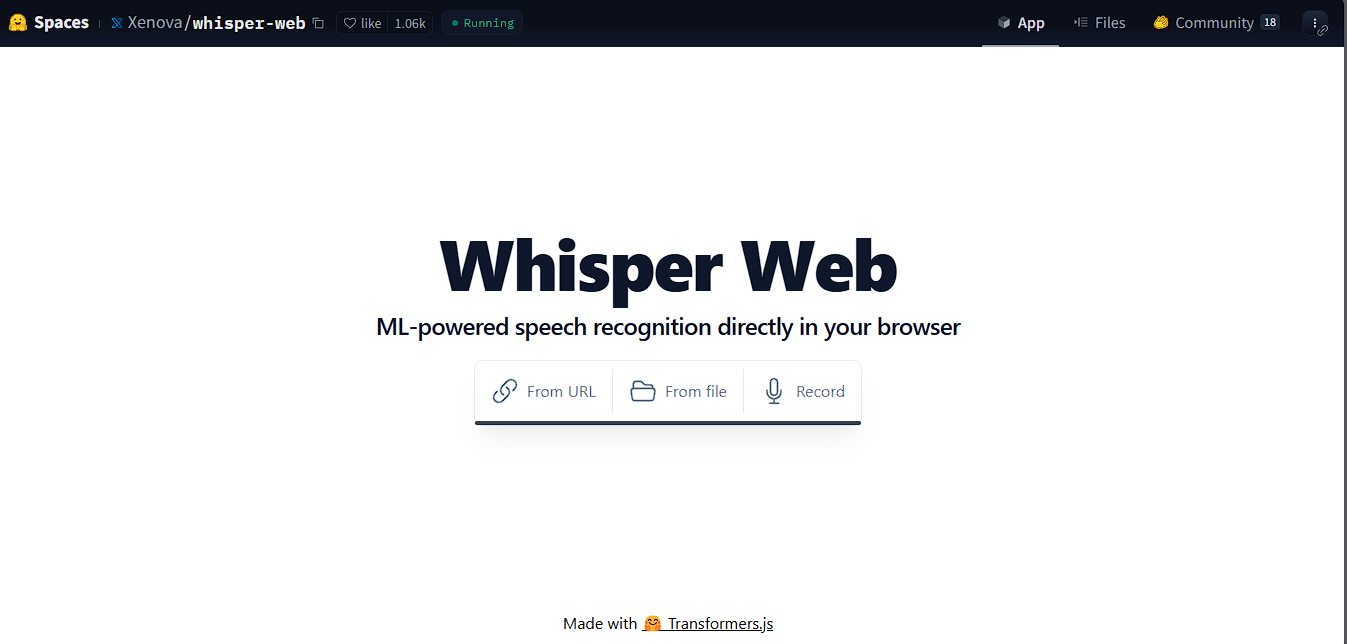
\includegraphics[width=0.8\linewidth]{img/WhisperWeb.png}
    \caption{Whisper Web}
    \label{fig:WhisperWeb}
\end{figure}

En la Figura~\ref{fig:WhisperWeb} se muestra un proyecto de la comunidad que busca llevar Whisper al navegador, sin la necesidad de un back-end. Para ello se usan tecnologías como:
\begin{itemize}
  \item WebAssembly (WASM): para correr código pesado directamente en el navegador.
  \item ONNX (Open Neural Network Exchange): para convertir modelos de PyTorch a un formato más portable.
  \item WebGPU o WebGL: para aprovechar el hardware del usuario (si es compatible).
\end{itemize}

Para ello se da uso a la plataforma y comunidad de Huggind Face enfocada en el desarrollo, distribución y uso de modelos de inteligencia artificial. 

El funcionamiento en esta aplicación web es el siguiente: 
\begin{itemize}
  \item Se carga un archivo de audio o se graba la voz.
  \item En el navegador elige una versión comprimida del modelo Whisper y la elección del lenguaje si el usuario lo desea.
  \item El modelo se ejecuta localmente en el navegador (no sube tu audio a la nube).
  \item La app procesa el audio y muestra la transcripción en pantalla.
  \item El navegador puede exportar la información.
\end{itemize}
Esta idea se descartó debido a la complejidad de implementación en el navegador, ya que ejecutar modelos de reconocimiento de voz como Whisper directamente en la web implica múltiples desafíos técnicos. Entre ellos destacan el alto consumo de recursos, la falta de soporte en entornos como WebAssembly/WebGPU, y la necesidad de transcribir y optimizar los modelos para que puedan ejecutarse localmente en el cliente sin afectar la experiencia del usuario.

Además, el peso de los modelos de en sus versiones más pequeñas, puede afectar significativamente los tiempos de carga y procesamiento, especialmente en dispositivos móviles o con hardware limitado. Por estas razones, se optó por explorar soluciones alternativas que pudieran integrarse de manera más eficiente dentro del proyecto.


\subsection{Web Speech API}

La principal tecnología nativa para reconocimiento de voz directamente en los navegadores es la Web Speech API, específicamente su interfaz SpeechRecognition.

La Web Speech API fue introducida como un borrador por el W3C (World Wide Web Consortium) en 2012. Aunque algunas partes de la API, como la síntesis de voz (SpeechSynthesis), han alcanzado un estado de recomendación, la parte de reconocimiento de voz (SpeechRecognition) aún se considera un borrador de trabajo. Sin embargo, ha sido implementada en la mayoría de los navegadores modernos, aunque con diferentes niveles de soporte y posibles requisitos de prefijos específicos del navegador (ej.: webkitSpeechRecognition en Chrome), por ejemplo el uso de esta API en navegadores específicos para gafas VR/AR como las Quest3 es directamente imposible, debido a que no hay soporte para ello, por esto lo más factible para el uso de reconocimiento de voz en casos como estos es usar un back-end que reciba las peticiones y chuncks de audio del cliente y está mismo las transcriba devolviendo así el texto transcrito.

El uso principal que le daríamos para este proyecto será el 'SpeechRecognition' para convertir la voz en texto. Es cierto que la compatibilidad de navegadores es muy grande, pero el soporte de SpeechRecognition no es estándar aún, y muchos navegadores solo lo permiten con el prefijo webkit (webkitSpeechRecognition). Funciona principalmente en Chrome y navegadores basados en Chromium, como se ve en la Figura~\ref{fig:SpeechRecognitionAPI}.

\begin{figure}[H]
    \centering
    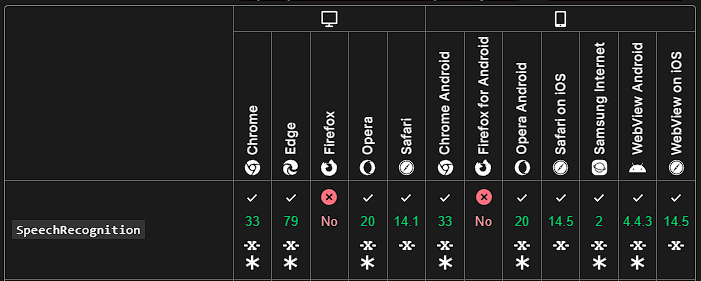
\includegraphics[width=0.8\linewidth]{img/WebSpeechAPI.png}
    \caption{Compatibilidad en exploradores}
    \label{fig:SpeechRecognitionAPI}
\end{figure}

Finalmente, una de las razones por las que se optó por esta opción es su facilidad de implementación, ya que no requiere de librerías externas, se ejecuta directamente en el navegador y es ideal para el uso de prototipos, demos o apps ligeras.

\begin{figure}[H]
    \centering
    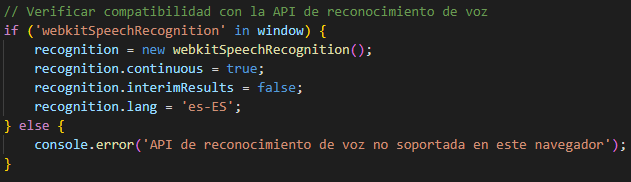
\includegraphics[width=0.8\linewidth]{img/WebKit.png}
    \caption{Ejemplo basico de WebSpeechAPI}
    \label{fig:WebKit}
\end{figure}

Como se observa en la Figura~\ref{fig:WebKit} la integración se hace en pocas líneas de código. Este código muestra la activación de reconocimiento continuo \textbf{'recognition.continuous = true; '}, esto quiere decir que se procesara la transcripción continuamente, pero con la condición de devolver el resultado final gracias a \textbf{'recognition.interimResults = false; '} además de seleccionar el idioma que se desea transcribir.

Por otro lado, no todas son ventajas, existen limitaciones para el uso de esta API, tales como el requerimiento de conexión a internet, ya que utiliza los servidores de Google para el reconocimiento. Además, el soporte y el comportamiento pueden variar entre diferentes navegadores. Y sobre todo, cuenta con una menor precisión en comparación con modelos como Whisper, especialmente en ambientes ruidosos o con acentos fuertes.


\subsection{AssemblyAI}

Assembly AI\footnote{Documentacion de Assembly~\cite{assemblyai_about}.} es una plataforma de Inteligencia Artificial que ofrece potentes APIs para el procesamiento de audio, incluyendo reconocimiento de voz (Speech-to-Text), comprensión del lenguaje natural (NLP) y otras funcionalidades de inteligencia de audio.

Cuenta con características similares a Web Speech API, salvo que tiene algunas mejoras en otros puntos.

Assembly AI se enfoca en ofrecer modelos de reconocimiento de voz de última generación entrenados en grandes cantidades de datos, lo que generalmente resulta en una mayor precisión, especialmente en entornos ruidosos o con acentos variados, con la posibilidad de identificar al hablante, detectar las emociones expresadas en el audio, incluso admite diferentes formatos de archivo y fuentes de audio/video que puedes ser en tiempo real o no.

La API es robusta y escalable, fue diseñada para desarrolladores que necesitan integrar capacidades de reconocimiento de voz en aplicaciones complejas y a gran escala. Por ello al ser una API externa, funciona de manera consistente en diferentes navegadores y plataformas, su uso en navegadores se realizará a través de una API REST y las respuestas se reciben como respuesta a dicha API por esto requiere una conexión a internet activa para enviar y recibir datos de la API. Assembly AI es un servicio comercial y tiene costos asociados en función del volumen de audio procesado, aunque a menudo ofrecen planes gratuitos o de prueba.

Finalmente, usamos esta tecnología para el proyecto en una segunda demo para el uso de gafas VR/AR, debido a que los navegadores de Meta de las gafas de pruebas no soportaban el manejo de la API anterior de Web Speech Recognition.

\cleardoublepage
\section{A-Frame} 
\label{sec:seccion2}

Para la implementación en AR/VR se uso A-Frame\footnote{Véase la página de referencia de A-Frame~\cite{aframe2025}.}, este es un framework web de código abierto usado para el desarrollo de experiencias en realidad virtual y aumentada. Utilizando HTML como lenguaje principal para la definición de escenas. Este framework se basa en Three.js, el cual es una biblioteca de JavaScript para gráficos en 3D.

A-Frame se caracteriza por el uso simplificado de Three.js para la creación de escenas, evitando el directo y complejo gestionamiento de los detalles de renderización en 3D.

Usando una arquitectura llamada ECS (Entity Components System) que es aplicada a los videojuegos, en donde cada objeto es una entidad diferenciada, que puede o no albergar otras entidades. Debemos tener en cuenta que para acceder a la librería de este framework debemos usar la línea de código del Listing~\ref{lst:acceso_A-Frame}. Esta etiqueta \texttt{<script>} permite cargar la versión 1.7.0 de A-Frame directamente desde la web. Dicha versión puede variar.
\begin{lstlisting}[language=HTML, caption=Línea de código de A-Frame, captionpos=b,label=lst:acceso_A-Frame]
  <script src='https://aframe.io/releases/1.7.0/aframe.min.js'></script>
\end{lstlisting}

Una de las características más claras de A-Frame es la definición de entidades utilizando un etiquetado similar al de HTML. Esto permite a desarrolladores construir mundos virtuales de manera rápida y simple, como se observa en este fragmento de código del Listing~\ref{lst:a-scene_Figure}: 


\begin{lstlisting}[language=HTML, caption=Escena A-Frame básica, captionpos=b,label=lst:a-scene_Figure]

      <a-scene>
        <a-box position='-1 0.5 -3' rotation='0 45 0' color='#4CC3D9'></a-box>
        <a-sphere position='0 1.25 -5' radius='1.25' color='#EF2D5E'></a-sphere>
        <a-cylinder position='1 0.75 -3' radius='0.5' height='1.5' color='#FFC65D'></a-cylinder>
        <a-plane position='0 0 -4' rotation='-90 0 0' width='4' height='4' color='#7BC8A4'></a-plane>
        <a-sky color='#ECECEC'></a-sky>
      </a-scene>
\end{lstlisting}

Cada entidad de esta escena tiene sus propiedades especificadas en la página de la documentación de A-Frame\footnote{Véase la documentación de A-Frame~\cite{aframe2025docs}.}

\begin{figure}[H]
    \centering
    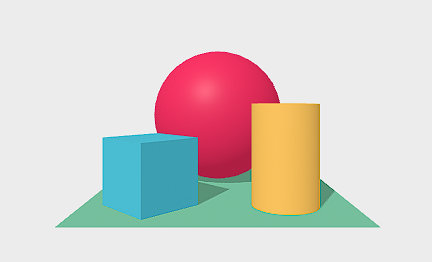
\includegraphics[width=0.5\linewidth]{img/SceneSimple.png}
    \caption{Escena simple A-Frame}
    \label{fig:aframe-scene}
\end{figure}

El núcleo de A-Frame es su sistema de entidades-componentes. Las entidades son objetos genéricos que adquieren propiedades y comportamientos mediante componentes. Los componentes son módulos reutilizables que añaden comportamientos, propiedades visuales, interacciones y varias acciones más a las entidades. A-Frame proporciona componentes predefinidos (position, rotation, scale, material, geometry\ldots). Se puede observar en el Listing~\ref{lst:componente}, el componente añade una entidad con un \texttt{<a-text>} que dará una información al usuario.

\begin{lstlisting}[language=HTML, caption=Crear Componente, captionpos=b, label=lst:componente]
  AFRAME.registerComponent('text-message', {
    init: function () {
        const userMessage = document.createElement('a-text');
        userMessage.setAttribute('id', 'userMessage');
        userMessage.setAttribute('value', 'Bienvenido a VOICE VR');
        userMessage.setAttribute('align', 'center');
        userMessage.setAttribute('color', 'black');
        userMessage.setAttribute('position', '0 20 -45');
        userMessage.setAttribute('width', '25');
        userMessage.setAttribute('look-at', '[camera]');
        this.el.appendChild(userMessage);
    }
});
\end{lstlisting}

Una entidad puede tener muchos componentes a la vez. Se pueden modificar los valores de un componente en tiempo real usando JavaScript. La creación de componentes depende de varias cosas como:
\begin{itemize}
  \item \textbf{Definición del componente:} Se realiza utilizando el método \texttt{AFRAME.registerComponent}.
  
  \item \textbf{schema:} Define los datos que el componente puede recibir, como configuraciones o parámetros personalizables.
  
  \item \textbf{init():} Función que se ejecuta al iniciar el componente. Se utiliza para establecer comportamientos iniciales o escuchar eventos de la escena.
  
  \item \textbf{this.el:} Hace referencia a la entidad (\texttt{<a-entity>}) sobre la cual está aplicado el componente.
\end{itemize}

\cleardoublepage
\section{Three.js} 
\label{sec:seccion3}

Como mencionamos anteriormente, A-Frame se construye sobre la potente biblioteca de gráficos 3D Three.js\footnote{Learning Three.js: The 
JavaScript 3D Library for 
WebGL~\cite{dirksen2013learning}.} el cual es una biblioteca de JavaScript que facilita la creación de gráficos 3D. A-Frame abstrae la complejidad de Three.js, permitiendo a los desarrolladores centrarse en la creación de contenido sin tener que lidiar directamente con la configuración de WebGL, shaders, matrices, etc. Sin embargo, para necesidades más avanzadas, los desarrolladores pueden acceder directamente al objeto Three.js subyacente dentro de los componentes personalizados de A-Frame.
Con Three.js, puedes crear y manipular formas básicas como cubos o esferas, importar modelos complejos (en formatos como GLTF), aplicar materiales y texturas, e iluminar escenas con luces realistas. Además, incluye cámaras y controles intuitivos para navegar, así como soporte para animaciones fluidas. 

La construcción de escenas mediante Three.js utilizará componentes como:

\begin{itemize}
    \item \textbf{Escena (Scene)}: el contenedor de todos los elementos 3D, como objetos, luces y cámaras.
    
    \item \textbf{Cámara (Camera)}: define el punto de vista desde el que se observa la escena. Las más comunes son la cámara de perspectiva y la ortográfica.
    
    \item \textbf{Renderizador (Renderer)}: convierte la escena y la cámara en una imagen visible en el lienzo HTML (\texttt{<canvas>}), usando WebGL.
    
    \item \textbf{Objetos (Mesh)}: representan modelos 3D, creados a partir de geometrías (formas básicas como cubos, esferas, planos, etc.) y materiales (color, textura, iluminación).
    
    \item \textbf{Luces (Light)}: iluminan la escena y permiten que los materiales reaccionen visualmente según el tipo de luz aplicada.
\end{itemize}


\cleardoublepage
\section{WebXR} 
\label{sec:seccion4}
Contextualizando este apartado debemos conocer la historia y desarrollo de WebXR. Fue desarrollada bajo las especificaciones del consorcio de W3C (World Wide Web)\footnote{WebXR según W3C~\cite{w3c_webxr}.}.

Su predecesor fue WebVR

'WebVR is an open specification that makes it possible to experience immersive virtual reality in your browser.'\footnote{WebVR según W3C ~\cite{webvr-spec}.} 

Esta era una API experimental creada únicamente para el desarrollo en realidad virtual. Este estándar fue algo fundamental para el desarrollo actual, pero presentaba varias limitaciones, ya que no abordaba los problemas relacionados con la realidad aumentada. La evolución y la integración de la realidad aumentada es la que creó el actual WebXR.

WebXR(Web Extended Reality) es un conjunto de tecnologías web que permite crear experiencias en realidad virtual (VR) y en realidad aumentada (AR) dentro de navegadores. Esto implica que cualquier usuario puede acceder a estas experiencias sin necesidad de descargar aplicaciones separadas.

WebXR presenta varias funcionalidades como: 

\begin{itemize}
  
 \item \textbf{Renderizado de Escenas 3D:} Facilita el renderizado de escenas 3D en estos dispositivos a las velocidades de fotogramas adecuadas, creando que la experiencia sea inmersiva.
 
 \item \textbf{Seguimiento de Movimiento:} WebXR puede rastrear el movimiento y la orientación de la cabeza y los controladores del usuario, lo que permite la interactividad.
 
 \item \textbf{Manejo de Entrada:} Admite la entrada de varios controladores y dispositivos XR, lo que permite la interacción del usuario.

\end{itemize}
Estas funcionalidades mencionadas más otras, crean las beneficiosas características que hacen que a este tipo de tecnologías web sean accesibles y compatibles en diferentes plataformas, aprovechando las diferentes tecnologías web familiares como JavaScript, HTML y WebGL para crear experiencias WebXR.

\cleardoublepage
\section{WebGL} 
\label{sec:seccion5}

WebGL surgió por la necesidad de llevar los gráficos 3D directamente a un navegador. Antes de que los gráficos 3D se limitaban a tecnologías basadas en plugins como 'Adobe Flash' o renderización puramente con JavaScript, esto resultaba en una caída abrupta de rendimiento.

Creada en 2007 por el grupo Khronos\footnote{Khronos Group ~\cite{webgl-khronos}.} fue desarrollada basándose en una API conocida como OpenGL ES 2.0 diseñada para dispositivos embebidos.

\textit{'WebGL is an API that brings hardware-accelerated 3D graphics to the Web, leveraging the widely adopted OpenGL ES 2.0 standard.' \cite{webgl-khronos}}

Esta tecnología fue impulsada gracias a empresas como Mozilla y Google, quienes fueron actores clave para la implementación y desarrollo del WebGL.

Una de las características más importantes de WebGL es la capacidad de aprovechamiento de la GPU de los dispositivos del usuario, permitiendo una renderización más rápida y eficiente de gráficos en 3D. Por otro lado, la integración en el DOM junto con otras tecnologías web como HTML, CSS y JavaScript ayudan al desarrollo de escenas en 3D como la Figura~\ref{fig:fishWebGL}. 
La multiplataformeidad que ofrece WebGL permite que se pueda ejecutar en cualquier navegador, independientemente de su sistema operativo.
\begin{figure}[H]  % Puedes quitar la opción [H] si no necesitas que esté en esa posición exacta
  \centering
  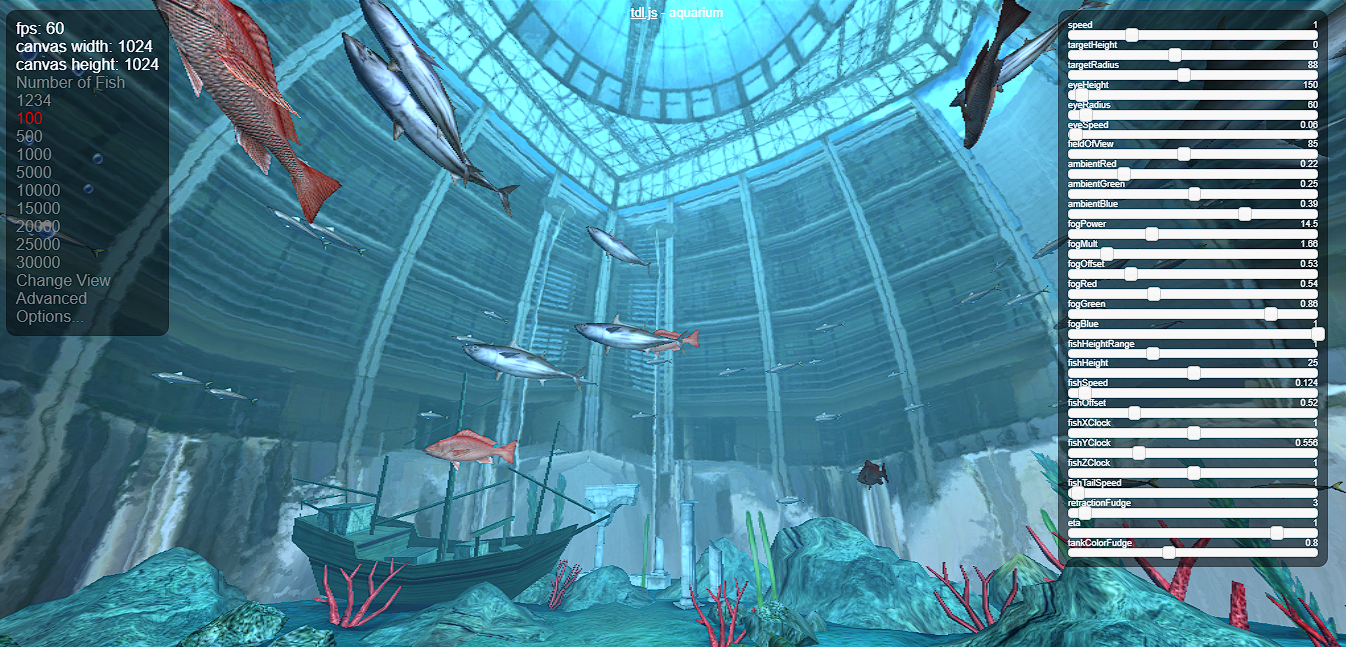
\includegraphics[width=0.8\linewidth]{img/WebGL.png}  % Ajusta el tamaño con width o height
  \caption{Ejemplo aplicacion en WebGL}  % Opcional: agrega una leyenda a la imagen
  \label{fig:fishWebGL}  % Opcional: añade una etiqueta para referenciar la imagen
\end{figure}
\cleardoublepage

\section{HTML} 
\label{sec:seccion6}

HTML(HyperText Markup Language) fue inventado por Tim Berners-Lee en el CERN (Organización Europea para la Investigación Nuclear) a principios de la década de 1990. Se buscaba que los científicos pudieran compartir información fácilmente a través de una red, en donde el hipertexto de HTML\footnote{HTML W3C ~\cite{w3c-html-intro}.} jugaba una parte esencial.

\textit{'HTML (HyperText Markup Language) is the set of markup symbols or codes inserted in a file intended for display on a World Wide Web browser page. The markup tells the web browser how to display a web page's words and images for the user.'} \cite{w3c-html-intro}

Esta definición de W3C muestra el propósito del HTML. A medida que la web evolucionó, HTML también lo hizo creando diferentes versiones que se iban adaptando al uso de navegadores.

La versión más moderna versión, el HTML5, introdujo una gran cantidad de características, como el soporte multimedia de audio y video, además de la posibilidad de Canvas para gráficos 2D.

El HTML como tal se conoce como lenguaje de marcado, lo que significa que utiliza etiquetas (tags) para estructurar el contenido. Estas etiquetas indican el significado y la presentación de diferentes elementos (encabezados, párrafos, imágenes, enlaces, etc.). Los documentos HTML cuentan con una estructura jerárquica basada en el anidamiento de elementos; esto permite introducir elementos o etiquetas dentro de otras, definiendo una relación entre dichos objetos de 'Padre-Hijo'. HTML5 introdujo elementos semánticos como:

La mayoría de las etiquetas usadas en HTML se deberán cerrar tras su uso.
\cleardoublepage
\section{JavaScript} 
\label{sec:seccion7}

'JavaScript es un lenguaje de programación interpretado que permite implementar funcionalidades complejas en páginas web, haciéndolas más dinámicas e interactivas.' \cite{mdn_javascript_intro_es}

Diseñado originalmente para ejecutarse en el navegador del cliente (front-end). Se caracteriza por la posibilidad de ser ejecutado línea a línea por el navegador, sin tener que compilarse antes de ello, además al ser un lenguaje de alto nivel facilita la escritura y comprensión de código, además también cuenta con un tipado de variables lo que significa que dichas 'variables' pueden cambiar a lo largo de la ejecución. 
Hoy en día también se usa en el lado del servidor (back-end) con entornos como Node.js, así como en desarrollo de aplicaciones móviles y de escritorio.

\subsection{Cliente (front-end)}
En el lado del cliente, JavaScript\footnote{Estructura de JavaScript~\cite{mdn_javascript_data_structures}.} permite manipular el DOM (Document Object Model), gestionar eventos del usuario, y hacer peticiones asincrónicas al servidor (AJAX o Fetch API), lo que lo convierte en una herramienta fundamental para crear experiencias de usuario dinámicas y reactivas. También ofrece acceso a diversas APIs del navegador que permiten funcionalidades avanzadas como geolocalización, almacenamiento local, gráficos mediante Canvas o WebGL, y comunicación en tiempo real con WebSockets o WebRTC.
\subsection{Servidor (back-end)}
En el entorno del servidor, JavaScript ha cobrado gran relevancia gracias a Node.js, que permite ejecutar código JavaScript fuera del navegador. Con Node.js es posible crear servidores web completos, manejar bases de datos y demás acciones. Su uso potenciado por npm (Node Package Manager), ofrece miles de módulos reutilizables para acelerar el desarrollo.

JavaScript juega un papel fundamental en el desarrollo de páginas web dinámicas, dotando al HTML antes mencionado con diferentes posibilidades de acción.

A lo largo del desarrollo del proyecto se ha usado en diferentes escenarios, desde la creación de un servidor simple, hasta la codificación de componentes para A-Frame con la finalidad de dar funcionalismo a escenas en 3D desarrolladas en dicho framework. 


\cleardoublepage
\section{CSS} 
\label{sec:seccion8}
CSS (Cascading Style Sheets) es como la cobertura y la decoración de una página web (el HTML sería el esqueleto). Se usa para decirle al navegador cómo mostrar los elementos de HTML: qué colores usar, qué fuentes, cómo se deben organizar en la pantalla, si deben tener márgenes, bordes, etc. 
Gracias a CSS, es posible crear interfaces web atractivas, responsivas y coherentes en distintos dispositivos.
Para su uso se podrá utilizar de la siguiente forma:

    \begin{table}[H]
      \centering
      \renewcommand{\arraystretch}{1.5}
      \begin{tabularx}{\linewidth}{|>{\centering\arraybackslash}p{2.5cm}|X|>{\centering\arraybackslash}p{0.28\linewidth}|}
      \hline
      \textbf{Método} & \textbf{Descripción} & \textbf{Ejemplo Visual} \\
      \hline
      
      \texttt{Inline} &
      Se aplica directamente en el atributo \texttt{style} de un elemento HTML. Útil para aplicar estilos rápidos. &
      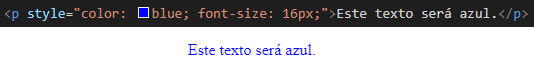
\includegraphics[width=0.9\linewidth]{img/style1.png} \\
      \hline
      
      \texttt{Internal} &
      Se define dentro del bloque \texttt{<style>} en la sección \texttt{<head>} del HTML. &
      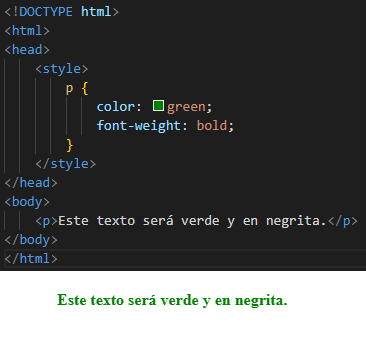
\includegraphics[width=0.9\linewidth]{img/Style2.png} \\
      \hline
      
      \texttt{External} &
      Consiste en enlazar un archivo externo con extensión \texttt{.css} mediante \texttt{<link>}. Es la forma más escalable. &
      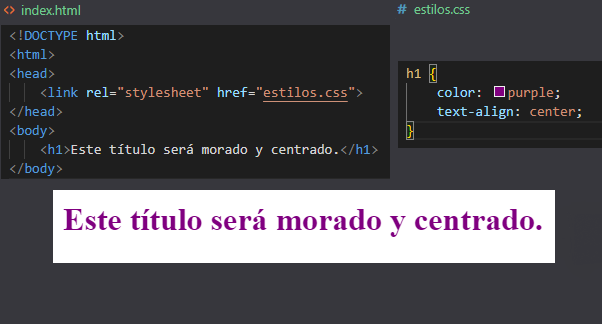
\includegraphics[width=0.9\linewidth]{img/Style3.png} \\
      \hline
      \end{tabularx}
      \caption{Formas de aplicar CSS en un documento HTML}
      \label{tab:formas-css}
      \end{table}
  Esta tecnología la usamos particularmente en una sección en la que mezclamos un HTML con estilos dentro de un panel de A-Frame conocido como 'HTML Embed Component' \footnote{HTML Embed Component information~\cite{aframeComponent}}.

\cleardoublepage

\section{NodeJS} 
\label{sec:seccion9}

Node.js es un entorno de ejecución de JavaScript de código abierto y multiplataforma. Permite ejecutar código JavaScript fuera de un navegador web.

Node.js fue creado por Ryan Dahl y se lanzó inicialmente en 2009. Se estaba buscando una forma más eficiente de manejar conexiones y concurrencia en la web después de experimentar problemas con el servidor web Apache. Se inspiró en lenguajes orientados a eventos y propuso una arquitectura basada en un bucle de eventos no bloqueante. La clave de esto fue la utilización del motor V8 presente en Google Chrome, el cual compila JavaScript de manera rápida y eficiente.

Node.js se centra en una arquitectura orientada a eventos y no bloqueante. Esto significa que, en lugar de esperar a que una operación de entrada/salida (E/S) se complete (bloqueando el hilo), Node.js registra una función de callback que se ejecutará una vez que la operación finalice. Esto permite manejar muchas conexiones simultáneas de manera eficiente con un solo hilo. 

Existen problemas con lo anterior mencionado; uno de los más importantes era el anidamiento de callback, ya que con un número excesivamente grande de estos, la lectura y mantención de estas se vuelven difíciles. Este problema se mitigó con la llegada de las promesas y las funciones \texttt{async/await}. También el uso de tareas complejas podría sobrecargar la CPU y afectar negativamente al hilo principal. 

\subsection{Node.js y el Manejo de Peticiones HTTP} 

Node.js es excelente para manejar peticiones HTTP, tanto para crear servidores web que responden a las solicitudes de los clientes (navegadores, otras aplicaciones) como para realizar peticiones a otros servidores (APIs externas).

\begin{itemize}
  \item \textbf{Módulo \texttt{http} y \texttt{https}:} Proporcionan las bases para crear servidores y clientes HTTP/HTTPS de bajo nivel.

  \item \textbf{Frameworks (Express):} Simplifican la creación de servidores web con funcionalidades para enrutamiento, middleware y gestión de solicitudes/respuestas.

  \item \textbf{Clientes HTTP:} Para realizar peticiones a otros servidores, se pueden usar los módulos nativos (\texttt{http}, \texttt{https}) o bibliotecas de terceros más convenientes como \texttt{axios} o \texttt{node-fetch}.

  \item \textbf{Manejo de Métodos HTTP:} Node.js facilita el manejo de diferentes métodos HTTP (\texttt{GET}, \texttt{POST}, \texttt{PUT}, \texttt{DELETE}, etc.) para construir APIs RESTful.

  \item \textbf{Streams:} Node.js utiliza \textit{streams} para manejar grandes cantidades de datos de manera eficiente durante las peticiones y respuestas, evitando cargar todo en la memoria.
\end{itemize}
\subsection{Certificados} 

Para asegurar las comunicaciones a través de la web (HTTPS), Node.js permite trabajar con certificados SSL/TLS.

\begin{itemize}
 \item \textbf{Módulo \texttt{https}:} El módulo \texttt{https} permite crear servidores HTTPS configurando las opciones del certificado (clave privada, certificado, certificados de autoridad \textit{CA} si es necesario).
 \item \textbf{Obtención de Certificados:} Los certificados se pueden obtener de autoridades de certificación (CA) como \textit{Let's Encrypt} (que ofrece certificados gratuitos) o de proveedores comerciales. También se pueden generar certificados autofirmados para entornos de desarrollo o pruebas (aunque no son confiables para producción).
 \item \textbf{Configuración del servidor:} Al crear un servidor HTTPS en Node.js, se deben especificar las rutas a los archivos del certificado y la clave privada en las opciones de configuración.
 \item \textbf{Manejo de Peticiones Seguras:} Una vez configurado el servidor HTTPS, Node.js manejará automáticamente el cifrado y descifrado de las comunicaciones.
 \item \textbf{Clientes HTTPS:} Al realizar peticiones HTTPS a otros servidores, Node.js maneja la verificación del certificado del servidor remoto (si está configurado correctamente con una CA de confianza).
\end{itemize}

\cleardoublepage
\section{Aplicaciones de inspiración al proyecto } 
\label{sec:seccion10}
El reconocimiento de voz y la creación de objetos está abriendo muchas posibilidades interesantes en diversas aplicaciones y juegos, incluyendo experiencias en gafas de realidad virtual (VR) y realidad aumentada (AR). Aquí te presento algunos ejemplos:

\subsection{Arkio:}

Arkio es una herramienta de diseño espacial colaborativo que permite a las personas crear y colaborar utilizando Realidad Virtual (VR), así como en PC, tablet y móvil.

\begin{figure}[H]  % Puedes quitar la opción [H] si no necesitas que esté en esa posición exacta
  \centering
  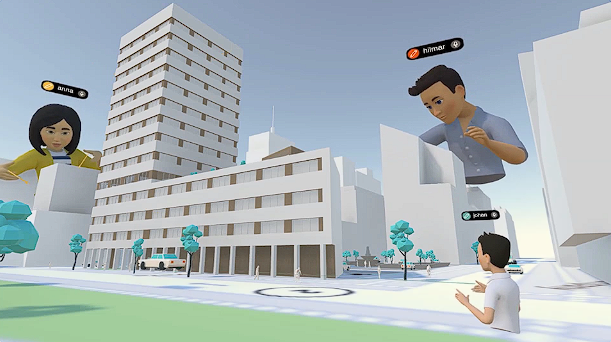
\includegraphics[width=0.8\linewidth]{img/arkio.png}  % Ajusta el tamaño con width o height
  \caption{Ejemplo de escena de Arkio}  % Opcional: agrega una leyenda a la imagen
  \label{fig:arkio}  % Opcional: añade una etiqueta para referenciar la imagen
\end{figure}

\begin{itemize}
  \item Se centra en el diseño de interiores, edificios, espacios virtuales y planificación urbana. 
  \item Facilita la colaboración multiplataforma en tiempo real como se ve en la Figura~\ref{fig:arkio}.
  \item Dispone de plugins para integrar con herramientas de diseño 3D como \texttt{Revit}, \texttt{Rhino} y \texttt{SketchUp}, permitiendo importar modelos existentes y exportar el trabajo realizado en Arkio.
  \item Arkio permite a los usuarios dibujar y manipular elementos arquitectónicos de forma intuitiva en el espacio VR mediante el uso de los mandos de que traen las gafas como la Quest3.
\end{itemize}

\subsection{VR Sculpting:}
VR Sculpting con Comandos de Voz: En la escultura VR (como en Shapelab Figura~\ref{fig:Shapelab} o Gravity Sketch), se han explorado o implementado (a menudo a través de plugins o herramientas de terceros como VoiceAttack) comandos de voz para tareas específicas durante el proceso de modelado. Estos comandos no forman parte nativa del software, pero permiten extender su funcionalidad, especialmente en contextos de accesibilidad, productividad o flujo de trabajo manos libres. Por ejemplo, podrías usar la voz para:
\begin{itemize}
    \item Seleccionar herramientas.
    \item Modificar parámetros.
    \item Realizar acciones.
\end{itemize}
Si bien esto no es la creación del objeto desde cero con la voz, sí permite una manipulación y modificación significativa mediante comandos hablados.
\begin{figure}[H]  % Puedes quitar la opción [H] si no necesitas que esté en esa posición exacta
  \centering
  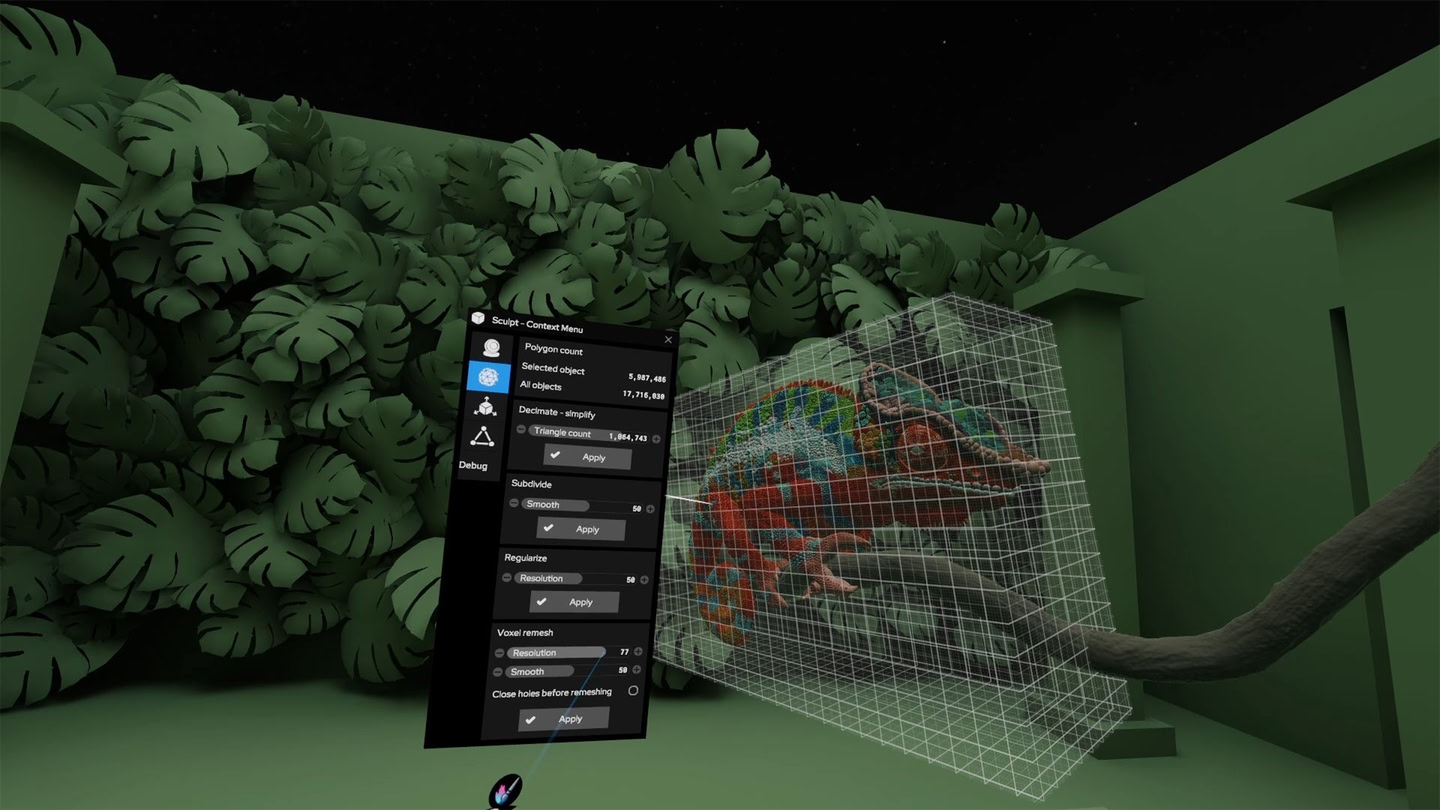
\includegraphics[width=0.8\linewidth]{img/Shapelab.jpg}  % Ajusta el tamaño con width o height
  \caption{Ejemplo de uso de Shapelab}  % Opcional: agrega una leyenda a la imagen
  \label{fig:Shapelab}  % Opcional: añade una etiqueta para referenciar la imagen
\end{figure}
\cleardoublepage
\subsection{Bridge Crew (Star Trek)}

Inicialmente, se añadió soporte para comandos de voz mediante la integración con IBM Watson, permitiendo a los jugadores emitir órdenes verbales a la tripulación en misiones para un solo jugador. Esta funcionalidad estaba disponible exclusivamente en inglés y requería el uso de un micrófono durante el juego, como se puede ver en la Figura~\ref{fig:startrek}.
Ubisoft desactivó esta característica debido a la finalización del contrato con IBM, lo que resultó en la eliminación del soporte de comandos de voz en todas las plataformas.

\begin{figure}[H]  % Puedes quitar la opción [H] si no necesitas que esté en esa posición exacta
  \centering
  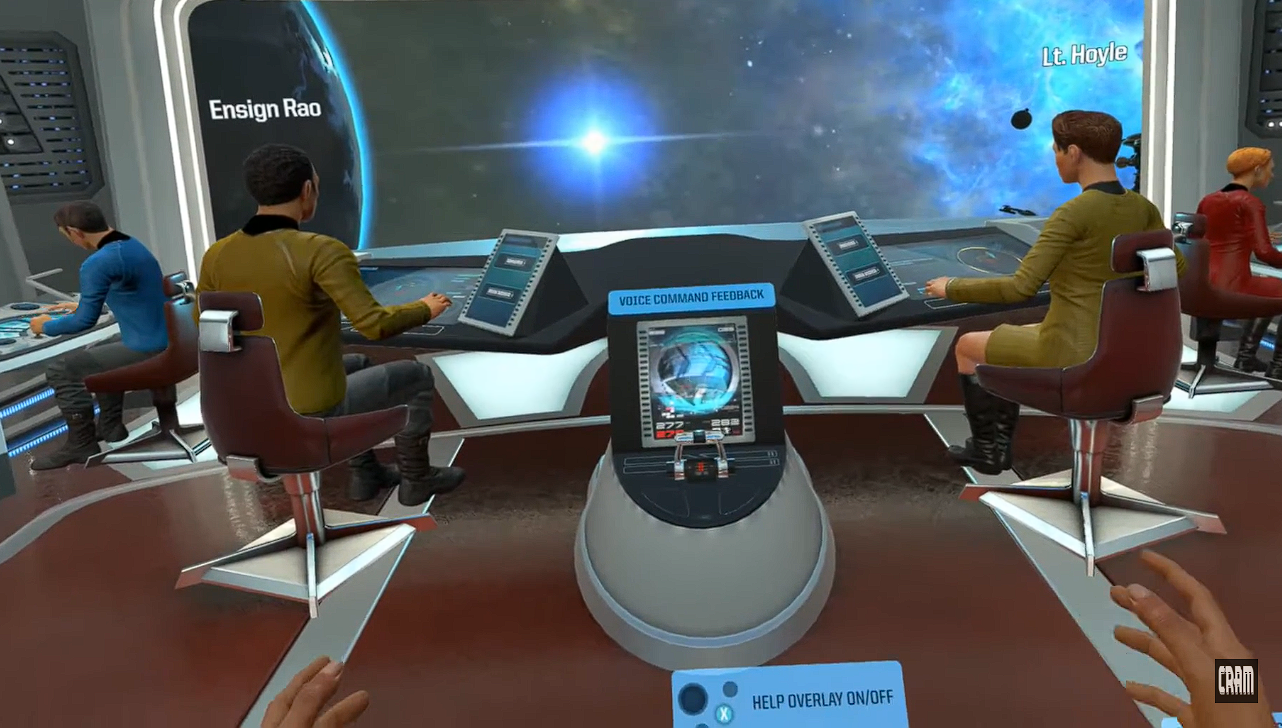
\includegraphics[width=0.8\linewidth]{img/startrek.png}  % Ajusta el tamaño con width o height
  \caption{Ejemplo de uso de Star Trek}  % Opcional: agrega una leyenda a la imagen
  \label{fig:startrek}  % Opcional: añade una etiqueta para referenciar la imagen
\end{figure}

Estas aplicaciones sirvieron como inspiración tanto por sus mecanismos de creación de objetos como por su capacidad para detectar y ejecutar comandos por voz. 
Este proyecto fue desarrollado con el objetivo de aprovechar esas funcionalidades, integrándolas en una sola herramienta accesible. 
El resultado en este proyecto busca combinar ambas facetas \textbf{creación y control por voz} en una plataforma accesible desde cualquier navegador web.

\cleardoublepage
\section{Tecnologias auxiliares} 
\subsection{Github}
GitHub se ha consolidado como la plataforma líder para el desarrollo colaborativo de software. 
Basándose en el sistema de control de versiones de Git, ofrece un entorno robusto para que desarrolladores de todo el mundo puedan trabajar simultáneamente en proyectos, gestionando los cambios de código de manera eficiente y organizada.

Su principal función radica en el alojamiento de repositorios, que actúan como almacenes centrales para el código fuente de un proyecto. Git permite rastrear cada modificación realizada en el código a lo largo del tiempo, facilitando la reversión a versiones anteriores, la identificación de la autoría de los cambios y la fusión del trabajo de diferentes colaboradores.
Las pull requests (solicitudes de extracción) sirven como mecanismo para proponer cambios, iniciar discusiones sobre el código y, finalmente, integrarlos a la rama principal.

Gracias a estas funcionalidades se ha ido desarrollando poco a poco el proyecto, del que se está hablando en este documento. Si bien no se explotó toda la funcionalidad que Github aporta, ha sido de gran ayuda para la recuperación de versiones anteriores y guardar avances.
\subsection{Visual Studio Code}
Visual Studio Code es un editor de código fuente con un gran equilibrio entre ligereza y potencia. Se distingue por su rendimiento rápido y su capacidad para manejar proyectos de gran envergadura sin comprometer la fluidez.
Una de sus características más destacadas es su soporte integrado para una amplia gama de lenguajes de programación, incluyendo JavaScript y Python entre otros. 

Para cada lenguaje, VS Code ofrece funcionalidades específicas como el resaltado de sintaxis, que facilita la lectura del código, además de constar con un sistema de autocompletado inteligente que sugiere código, muestra información sobre funciones y parámetros, y ayuda a prevenir errores.

La depuración integrada es otra funcionalidad clave, permitiendo a los desarrolladores ejecutar y analizar su código directamente desde el editor. Se pueden establecer puntos de interrupción, inspeccionar el valor de las variables y seguir la ejecución paso a paso para identificar y corregir errores de manera eficiente.

El Marketplace de extensiones ofrece una vasta colección de herramientas. En este proyecto se usaron extensiones como \textbf{Live Server} y \textbf{Live Preview} para visualizar los cambios en tiempo real que se hacen tanto en JavaScript como en cuerpo del archivo de A-Frame.

\subsection{Gafas Meta Quest3}
Las gafas de realidad virtual (VR) y realidad mixta (MR) de Meta. 
Ofrecen experiencias inmersivas en VR y la capacidad de superponer elementos virtuales en el mundo real (MR). 
Cuentan con mayor resolución, potencia y nuevas funcionalidades como passthrough a color de alta resolución y seguimiento de manos mejorado. 
\begin{figure}[H]  % Puedes quitar la opción [H] si no necesitas que esté en esa posición exacta
  \centering
  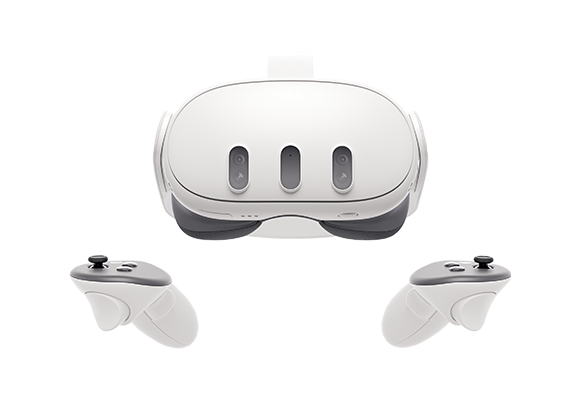
\includegraphics[width=0.8\linewidth]{img/Quest3.png}  % Ajusta el tamaño con width o height
  \caption{Gafas Meta Quest3}  % Opcional: agrega una leyenda a la imagen
  \label{fig:Quest3}  % Opcional: añade una etiqueta para referenciar la imagen
\end{figure}
Se utilizaron para hacer las pruebas de funcionamiento de la aplicación en los navegadores de Meta, pero contaba con ligeros problemas de compatibilidad para el uso de APIs que se usan en navegadores normales.
\subsection{LaTeX}

LaTeX, por otro lado, es un sistema de composición de textos de alta calidad, ideal para documentos técnicos. Se centra en la estructura y el contenido, dejando el formato en manos del sistema.

LaTeX automatiza la generación de elementos estructurales como la numeración de secciones, subsecciones, figuras y tablas. También se encarga de la creación automática de índices, bibliografías y referencias cruzadas, asegurando la coherencia y precisión en todo el documento. La salida final se caracteriza por su alta calidad tipográfica, gracias a los algoritmos de composición y al uso de fuentes profesionales.

Es usado para el desarrollo de la memoria del trabajo de fin de grado. Se tomó esta elección debido a que permite centrarse únicamente en el contenido textual, mientras que el sistema se encarga del diseño y formato del documento. 
\label{sec:seccion11}

\chapter{Desarrollo del proyecto}
\label{chap:Desarollo}
A este proceso se aplicaron estrategias basadas en metodologías ágiles. Para ser más preciso, se usó el método de Scrum para organizar el trabajo, un marco que facilita la gestión de proyectos complejos mediante ciclos iterativos conocidos como sprints. Hasta que no se consigue el objetivo de un sprint, no comienza el otro, y la consecución de los objetivos de todos los sprints coincide con la consecución del objetivo final del proyecto. Estos sprints a su vez se dividen en tareas mucho más pequeñas que persiguen objetivos más concretos y ayudan a la consecución del objetivo final del sprint.

Estructura mínima de cada sprint:
\begin{itemize}
\item Objetivos
\item Tareas Realizadas
\item Resultado
\item Lecciones aprendidas
\end{itemize}

\cleardoublepage

\section{Arquitectura general} 
\label{sec:arquitectura}



\begin{itemize}
  \item \textbf{Sprint 1: Investigación y Prototipado Inicial (3 semanas)}
 \begin{itemize}
  \item Investigación sobre uso, posible desarrollo y función de los objetos relacionados con el proyecto.
  \item Desarrollo e investigación de reconocimiento de voz.
  \item Desarrollo de la primera demo sobre funcionamiento de A-FRAME.
 \end{itemize}
 
 \item \textbf{Sprint 2: Desarrollo de A-FRAME Base (2 semanas)}
 \begin{itemize}
  \item Creación de objetos de A-FRAME simples.
  \item Creación de componentes para A-FRAME y reestructuración de código.
 \end{itemize}
 
 \item \textbf{Sprint 3: Funcionalidades y Componentes (2 semanas)}
  \begin{itemize}
   \item Creación de funcionalidades para componentes.
   \item Aumento de comandos para la funcionalidad del proyecto.
   \item Creación de escena simple para funcionalidaden escritorio
  \end{itemize}
 
 \item \textbf{Sprint 4: Mejora de componentes y Mejora Visual (2 semanas)}
  \begin{itemize}
   \item Crear componentes para editar y eliminar objetos.
   \item Mejora de la estética y colocación de objetos.
   \item Crear funcionalidad para nuevos componentes.
  \end{itemize}
 
 \item \textbf{Sprint 5: integración en VR/AR (1 semana)}
  \begin{itemize}
   \item Posibilidad de integración en VR/AR (Quest3).
   \item Creación de servidor privado.
  \end{itemize}
 
 \item \textbf{Sprint 6: Pasos finales (3 semanas)}
 \begin{itemize}
   \item Mejora la ética y posicionamiento de objetos en escena.
   \item Implementación de plugins extra para la visualización y decoraciones.
   \item Maquetado final de la demo para escritorio.
   \item Maquetado y unión del back-end y front-end para demo con gafas Quest3.
 \end{itemize}
\end{itemize}


\cleardoublepage
\section{Sprint 1} 
\label{sec:sprint1}
\textbf{Investigación y Prototipado Inicial}
El desarrollo de este primer Sprint tuvo una duración de 3 semanas, debido a que fue la primera toma de contacto con el servicio de reconocimiento de voz y del uso complejo en A-Frame.
Además, contamos con diferentes programas que se fueron desarrollando en el transcurso de este sprint. Estos programas se irán explicando a continuación. 
\subsection{Objetivos}
Los objetivos principales eran la recolección de información, datos y ejemplos de aplicaciones que pudieran ayudar al desarrollo de este proyecto, además de familiarizarnos más con los diferentes programas que se usarán en el desarrollo.
 \begin{itemize}
   \item Investigación del posible desarrollo, uso y funcionamiento de las tecnologías implicadas en el desarrollo del proyecto.
   \item investigación y desarrollo de ejemplos para reconocimiento de voz.
   \item Desarrollo de la primera demo sobre funcionamiento de A-FRAME.
 \end{itemize}

\subsection{Tareas Realizadas}

\begin{itemize}
 \item Gestionar información, ver ejemplos (si existen), buscar demos similares.
 \item Aplicar tecnologías de reconocimiento de voz y posibles usos.
 \item Desarrollo de demos iniciales para validar el uso de A-Frame con contenido dinámico.
\end{itemize}
\subsubsection{Aplicación de tecnologías de reconocimiento de voz}
Tras la recolección y análisis de información técnica relevante. 
Para ello, se harán pruebas con distintos sistemas de transcripción de voz. 
Y finalmente, se desarrollaron 3 ejemplos de cómo debía realizarse la funcionalidad para generar una transcripción.

\textbf{1. Reconocimiento de Voz en Python con Whisper}

Se utilizó el modelo \textbf{Whisper} de OpenAI en \textbf{local} para transcripción de audio. 
Este programa se llevó a cabo mediante Python, grabando la voz mediante el micrófono, y guardando el audio para luego usar Whisper en él y obtener una transcripción. 
%El gran problema que se encontro en ese momento fue la instalacion de Whisper en local, en cambio el uso de la API de OpenAI es muy facil ya que no necesitas la instalacion de ningun programa o libreria extra, tiene un coste.
%Tras la previa configuracion, las pruebas que se obtuvieron fueron relativamente malas, la latencia dependia mucho del modelo y el modelo en cambio dependia del hardware que se tuviera.
%La deteccion de palabras y acentos era muy consistente, haciendo que incluso con una mala grabacion de audio se obtuviera una transcripcion precisa.
%Este caso no permitia utilizarlo en navegadores ya que se basaba en un programa echo en Python.

\textbf{2. Servidor híbrido Node.js + Python}

Para el segundo caso, usamos un servidor propio creado a base de Node.js que se comunicaba con un el mismo script de Python en tiempo real para realizar las transcripciones del mismo modo que en el caso anterior.
Este caso se desarrolló para poder implementar la transcripción de voz en el navegador y desarrollar la idea principal del proyecto.
La transcripción obtenida se transmitiría al cliente web a través de WebSockets.
% REVISAR ESTE ENLACE DESPUÉS DE ARREGLAR EL REPOSITORIO.
\footnote{Ejemplo disponible en GitHub: \url{https://github.com/R4CC00N/SpeechRecognition_in_Browser/blob/main/Sprint2/Pyhton/prueba_whisper.py}.}

\textbf{3. Reconocimiento en el navegador (Web Speech API)}

Como caso de uso final se encontró una API dedicada a los navegadores, Web Speech API dio paso a la transcripción rápida y efectiva. Es necesario recalcar que depende mucho de la calidad de audio, y el navegador.
Dio unos buenos resultados, además de que, en el contexto del proyecto, cumplía los estándares que se intentaban alcanzar con el reconocimiento y transcripción de voz.

\subsubsection{Contacto con A-Frame y reconocimiento de voz}
También se planteó el primer contacto con el framework haciendo unas demos sencillas en las que se dará uso a un \textbf{\texttt{<a-text>}}para mostrar texto dinámicamente.
\textbf{Demo – Reconocimiento de Voz + A-Frame}

En esta demo se trabajó con el reconocimiento de voz desde el navegador (usando `Web Speech API`).
De la tal manera que al pulsar el botón principal que aparece en la Figura~\ref{fig:Demo1V2} se activa el evento de detección de voz que obtendrá permisos para el uso del micrófono y este al detectar al usuario hablar transcribe la voz, todo esto dentro del mismo navegador, gracias al componente \textbf{'input-text'}. 
Tras la obtención de la transcripción, esta aparece automáticamente en el elemento \texttt{<a-text>} dentro de la escena.
La experiencia permite mostrar mensajes de voz directamente dentro de un entorno 3D.
Si se detectan palabras como crear, editar u otro texto, el fondo cambia de color
% REVISAR ESTE ENLACE DESPUES DE ARREGLAR EL REPOSITORIO.
\footnote{Demo disponible en GitHub: \url{https://r4cc00n.github.io/SpeechRecognition_in_Browser/Sprint3/v2_A-Frame.html}.}
\begin{figure}[H]  % Puedes quitar la opción [H] si no necesitas que esté en esa posición exacta
  \centering
  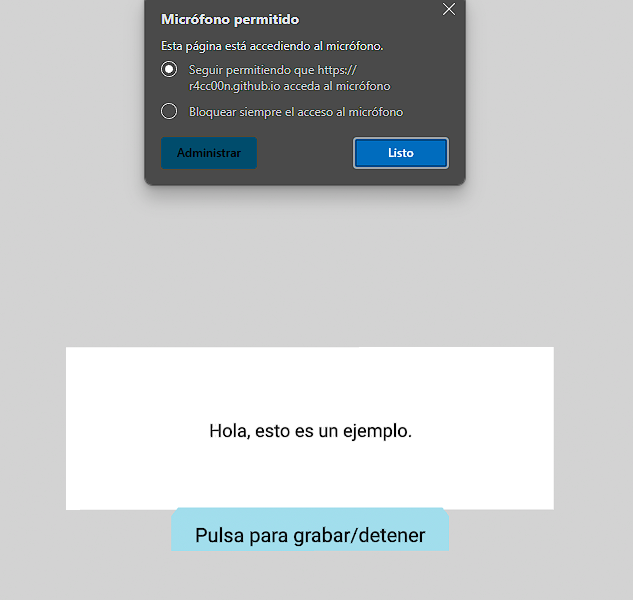
\includegraphics[width=0.5\linewidth]{img/Demo1_v2.png}  % Ajusta el tamaño con width o height
  \caption{Funcionamiento de la segunda Demo para A-Frame}  % Opcional: agrega una leyenda a la imagen
  \label{fig:Demo1V2}  % Opcional: añade una etiqueta para referenciar la imagen
\end{figure}  


\subsection{Resultados}

\textbf{Web Speech API:} es la solución más óptima para navegadores, aunque limitada en dispositivos VR se terminará usando en las demás demos.

\textbf{Demo - Reconocimiento de Voz + A-Frame: }Una vez conocidos los elementos a interactuar, el añadir un factor como el reconocimiento de voz fue un desafío de grado medio. Se encontró que la transcripción podía ser usada directamente para el cambio de valor dentro del \texttt{<a-text>}.

\subsection{Lecciones aprendidas}

\begin{itemize}
 \item Se concluyó que la opción \textbf{Web Speech API} fue la más eficiente y directa para pruebas en escritorio.
 También tuvo varias cosas negativas, la principal fue que en el uso de la detección y transcripción de voz en gafas de VR/AR, como son las Quest3, no fuesen soportadas en el navegador de Meta. 
 \item No obstante, esta incompatibilidad de \textbf{Web Speech API} con navegadores de gafas como la Quest3 llevó a plantear dos líneas de trabajo: una demo basada en navegador para escritorio, y una segunda demo soportada por back-end para su funcionamiento en gafas de realidad mixta, empleando Node.js y alguna API de reconocimiento de voz en el servidor.
\end{itemize}

\clearpage
%%% APARTIR DE AQUI LOS SPRINTS NECESITAN MAS DESAROLLO, DEJO COMENTADOS UNOS DATOS A COMPLETAR.
\section{Sprint 2} 
\label{sec:sprint2}
Este Sprint tuvo una duración de 2 semanas, además contiene \textbf{ demos interactivas} en las que se combina \textbf{A-Frame} con \textbf{reconocimiento de voz} para crear objetos 3D dentro de una escena usando comandos hablados.
Cada demo mejora la anterior, especialmente en el reconocimiento y manejo de \textbf{coordenadas y números}, permitiendo finalmente la creación precisa de objetos con posición y tamaño definidos por voz.
Además del incremento y mejoras en los \textbf{componentes} de A-Frame.

\subsection{Objetivos}
\begin{itemize}
  \item Implementación básica de reconocimiento de comandos de voz en una escena de A-Frame.
  \item Permitir la creación de objetos primitivos mediante comandos de voz.
  \item Implementar la capacidad de interpretar números en cifra tanto positivos como negativos.
  \item creación de componentes para A-FRAME y reestructuración de código.
\end{itemize}

\subsection{Tareas Realizadas}

\textbf{Demo - Comando Básico y Reconocimiento Inicial} 

En esta demo se creó un componente llamado \textbf{'input-text'} que, aparte de transcribir el audio, también detectará comandos de voz. 
Estos comandos serán procesados de la transcripción, como se puede ver en la Figura~\ref{fig:componente1}.
Trabajamos principalmente con el comando 'crear [objeto]', este permite la generación de cubos, solicitando a continuación la \textbf{'posición'} y el \textbf{'tamaño'} del objeto. 

Sin embargo, presenta ciertas limitaciones, una de ellas es la fiabilidad en el reconocimiento numérico (valores numéricos que la transcripción decide automáticamente poner como letras e incapacidad para interpretar valores números negativos en las transcripciones).
Otra de las limitaciones que encontramos es la captura de coordenadas como un bloque único
  \begin{figure}[H]  % Puedes quitar la opción [H] si no necesitas que esté en esa posición exacta
    \centering
    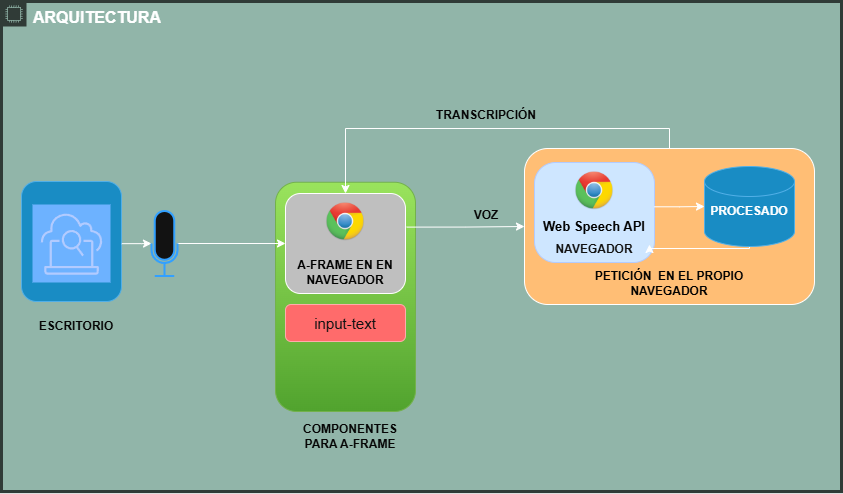
\includegraphics[width=0.7\linewidth]{img/componentes1.png}  % Ajusta el tamaño con width o height
    \caption{Flujo de creación de componentes}  % Opcional: agrega una leyenda a la imagen
    \label{fig:componente1}  % Opcional: añade una etiqueta para referenciar la imagen
  \end{figure} 

\textbf{Demo Final - Creación de Componentes en A-Frame y Reestructuración de Código}

Este sprint se centró en modulizar la escena en A-Frame mediante la creación de componentes reutilizables como se ve en la Figura~\ref{fig:componente2}, en ella se puede ver:
\begin{figure}[H]  % Puedes quitar la opción [H] si no necesitas que esté en esa posición exacta
  \centering
  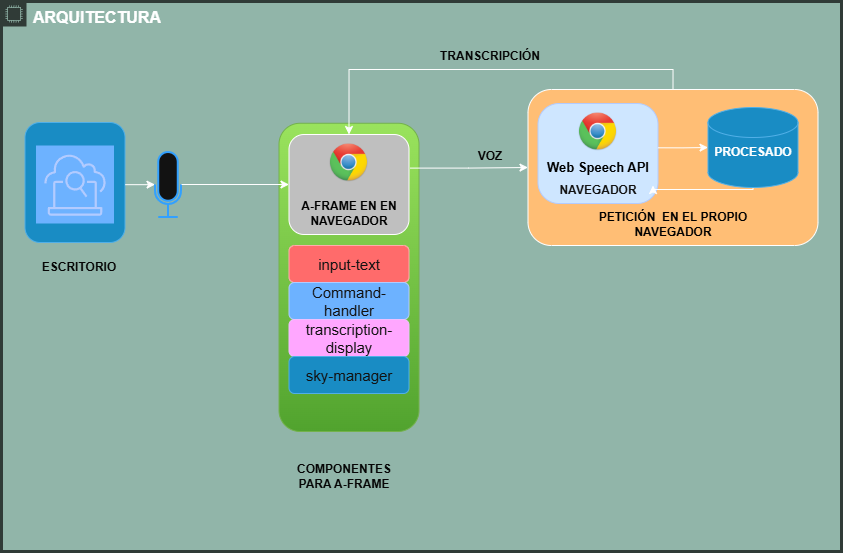
\includegraphics[width=0.7\linewidth]{img/componentes2.png}  % Ajusta el tamaño con width o height
  \caption{Flujo de creación de componentes avanzados}  % Opcional: agrega una leyenda a la imagen
  \label{fig:componente2}  % Opcional: añade una etiqueta para referenciar la imagen
\end{figure} 
\texttt{\textbf{command-handler:}} Es un componente que interpreta comandos de voz para crear objetos en la escena, pero con una entrada de audio configurable.
Además de aplicar una reestructuración del código con el fin de mejorar la organización, escalabilidad y mantenibilidad del proyecto.
Depende de que otro componente en la escena realice el reconocimiento de voz y emita un evento 'transcript' con el texto transcrito.
Durante su funcionamiento, emite eventos a nivel de escena (\texttt{enter-create-mode, exit-create-mode}) para señalar el inicio y el fin del proceso de creación.

\texttt{\textbf{transcription-display:}} Tiene la función de mostrar en un elemento de texto 3D con un \textbf{ID} definido (\texttt{<a-text>}) la transcripción de voz proveniente de otro componente de la escena.
Se puede observar su uso en la Figura~\ref{fig:comandDemo4} en donde aparecen los mensajes para el usuario en la parte superior de la caja de texto normal.


\texttt{\textbf{sky-manager:}} Se encarga de gestionar el color del fondo de la escena (\texttt{<a-sky>}) en respuesta a eventos personalizados emitidos a nivel de la escena provenientes del \texttt{\textbf{command-handler}}.

Añadido a estos componentes, decidimos deparar el código de \textbf{javascript} y el \textbf{HTML}, para organizar así mejor los archivos y la estructuración del proyecto.
También se han solucionado los problemas con los números creando un manejador de números.
\begin{figure}[H]  % Puedes quitar la opción [H] si no necesitas que esté en esa posición exacta
  \centering
  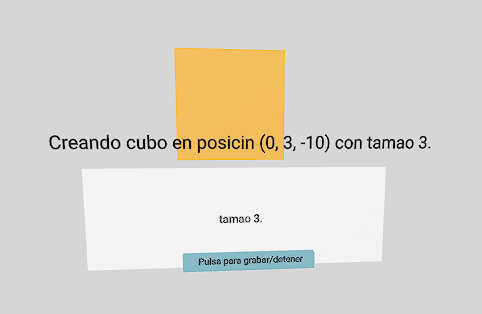
\includegraphics[width=0.7\linewidth]{img/comandoDemo4.png}  % Ajusta el tamaño con width o height
  \caption{Funcionamiento del comando basico Demo 4}  % Opcional: agrega una leyenda a la imagen
  \label{fig:comandDemo4}  % Opcional: añade una etiqueta para referenciar la imagen
\end{figure} 


\subsection{Resultados}
\begin{itemize}
 \item Se logró una implementación funcional del reconocimiento de voz para la creación de objetos 3D en un entorno A-Frame.
 \item Se demostró una mejora progresiva en la capacidad del sistema para comprender y procesar comandos de voz relacionados con la creación, posición y tamaño de objetos.
 \item La interacción para especificar la posición de los objetos evolucionó de una entrada de bloque (123) a una solicitud secuencial (x=1,y=2,z=3), mejorando la usabilidad.
 \item En la última demo, se implementó con éxito la interpretación de números tanto en formato numérico como en palabras, incluyendo valores negativos, lo que amplía la flexibilidad de la entrada por voz.
 \item Se proporcionó retroalimentación visual constante al usuario sobre el estado de la grabación y el texto reconocido a través de la interfaz en la escena.
 \item Se mejoró la legibilidad del texto al separar en diferentes archivos el JavaScript y el HTML.
\end{itemize}
\subsection{Lecciones aprendidas}
\begin{itemize}
 \item La creación de componentes en A-Frame facilita la organización y la reutilización de la lógica de la aplicación.
 \item La interpretación del lenguaje natural, incluso para tareas específicas, requiere una consideración cuidadosa de las posibles formas en que los usuarios pueden expresar sus comandos. El manejador para números es un ejemplo de cómo abordar esta complejidad.
 \item La retroalimentación visual es esencial para mantener al usuario informado y para depurar el proceso de reconocimiento e interpretación de voz.
 \item La iteración y la mejora progresiva, como se ve en la secuencia de los cuatro demos, es un enfoque efectivo para abordar desafíos técnicos.
\end{itemize}

\clearpage 
\section{Sprint 3} 
\label{sec:sprint3}
Este sprint tuvo una duración de 2 semanas, en donde se desarrolló las capacidades del proyecto, añadiendo más modificadores, creando componentes e incluso mejorando la división del código.
Durante el desarrollo de este Sprint se crearon componentes para el accionar del proyecto.
\subsection{Objetivos}
\begin{itemize}
 \item Creación de funcionalidades para componentes.
 \item Aumento de comandos para la funcionalidad del proyecto.
 \item Creación de escena simple para funcionalidad en escritorio.
\end{itemize}
\subsection{Tareas Realizadas}

\textbf{Demo - Creador de objetos funcionalidades }
\begin{figure}[H]  % Puedes quitar la opción [H] si no necesitas que esté en esa posición exacta
  \centering
  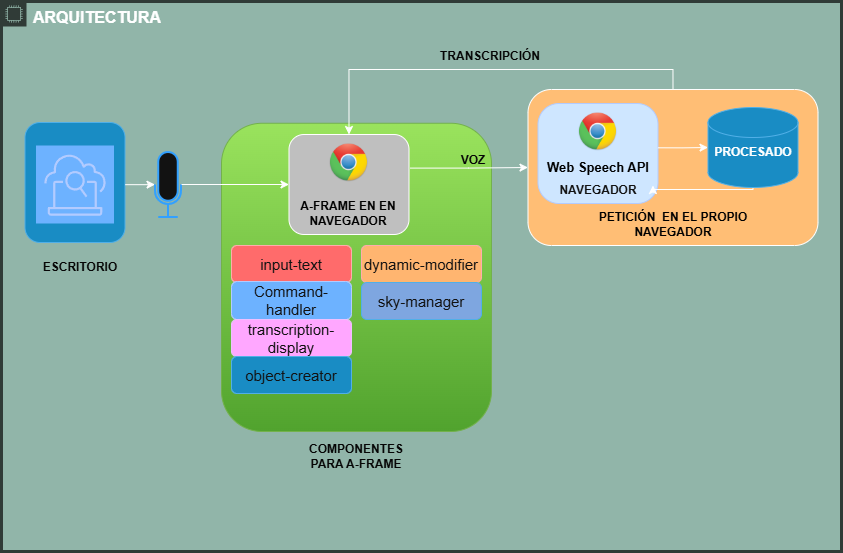
\includegraphics[width=0.6\linewidth]{img/componentes3.png}  % Ajusta el tamaño con width o height
  \caption{Flujo de creación de componentes avanzados}  % Opcional: agrega una leyenda a la imagen
  \label{fig:componente3}  % Opcional: añade una etiqueta para referenciar la imagen
\end{figure} 

\textbf{object-creator:} Escucha el evento \textbf{start-object-creation} y, basándose en el tipo de objeto recibido, crea la entidad con una geometría predefinida, una posición y rotación fijas.

\textbf{dynamic-modifier:} Este componente edita en tiempo real el objeto creado con diferentes funcionalidades de modificación Paso a Paso \textbf{(stepsPOS, stepCOLOR, stepID, stepSIZE)} para manejar la modificación de cada atributo de forma conversacional.

Se introduce una variable global \textbf{step} (inicializada en null). Esta variable se utiliza para gestionar un flujo de conversación paso a paso durante la modificación de los atributos (posición, tamaño, color, ID).


La palabra clave \textbf{'cambio'} ahora se utiliza para salir del modo de modificación.
Este cambio envía un mensaje al usuario que se utiliza para guiarlo a través del proceso de modificación.
\begin{figure}[H]  % Puedes quitar la opción [H] si no necesitas que esté en esa posición exacta
  \centering
  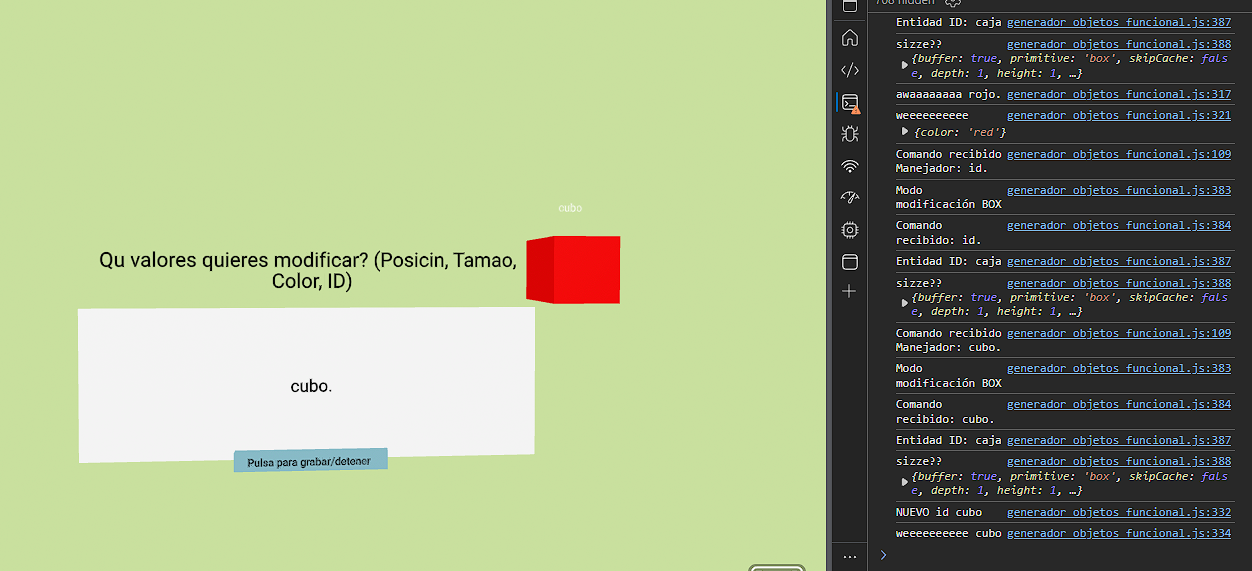
\includegraphics[width=0.6\linewidth]{img/generador_funcional_v1.png}  % Ajusta el tamaño con width o height
  \caption{Funcionamiento del generador de objetos con funcionalidades extra}  % Opcional: agrega una leyenda a la imagen
  \label{fig:generadorFuncionalDemo1}  % Opcional: añade una etiqueta para referenciar la imagen
\end{figure} 

\subsection{Resultados}

Este sprint implementó la interacción por voz para la gestión de objetos:

Se creó el componente \textbf{object-creator} para crear objetos básicos, el cual cumple relativamente bien su función.

Además, se implementó la \textbf{modificación conversacional} paso a paso de posición, color, ID y tamaño durante la creación del objeto.

La mayoría de estos componentes se mantendrán hasta la etapa final, solventando algunos fallos que pudieran encontrarse en ellos durante el desarrollo.

\subsection{Lecciones aprendidas}
\textbf{Componentes para modularidad:} Organizar la lógica en componentes facilita el desarrollo y mantenimiento.

\textbf{Gestión de estados en voz:} Las interacciones conversacionales requieren un seguimiento claro del estado.

\textbf{Asincronía de la voz:} La transcripción y respuesta necesitan manejar la latencia.

\textbf{Comandos de voz intuitivos:} El lenguaje claro y la guía mejoran la experiencia del usuario.

 \clearpage
\section{Sprint 4} 
\label{sec:sprint4}
Este Sprint tuvo una duración de 2 semanas, en donde se dieron la mayoría de los avances en creación de componentes, como se puede ver en la Figura~\ref{fig:componente4} .
\subsection{Objetivos}
\begin{itemize}
\item Crear componentes para editar y eliminar objetos creados.
\item Modificar la escena para mejor uso del usuario.
\item Crear comandos nuevos para la funcionalidad de los nuevos componentes.
\item Mejora de la estética y colocación de objetos.
\end{itemize}
\subsection{Tareas Realizadas}
\textbf{Demo - Nuevas funcionalidades}

\begin{figure}[H]  % Puedes quitar la opción [H] si no necesitas que esté en esa posición exacta
  \centering
  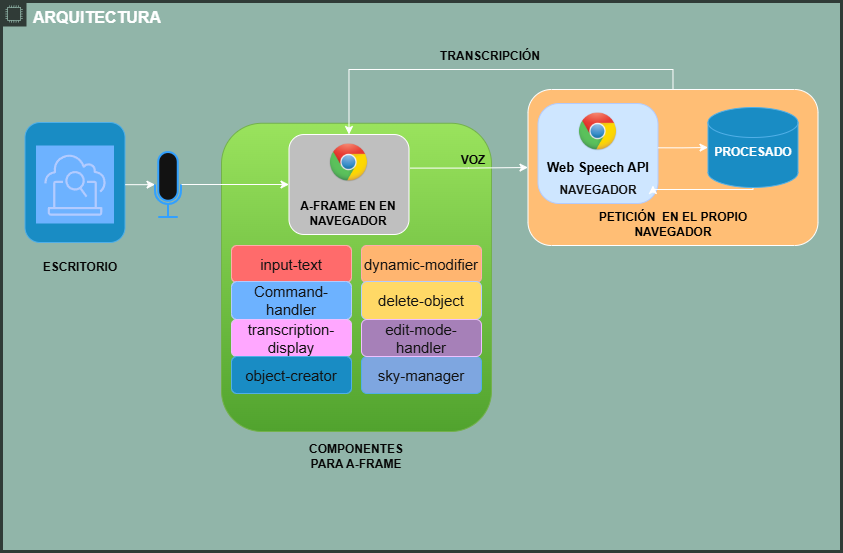
\includegraphics[width=0.6\linewidth]{img/componentes4.png}  % Ajusta el tamaño con width o height
  \caption{Flujo de creación de componentes avanzados}  % Opcional: agrega una leyenda a la imagen
  \label{fig:componente4}  % Opcional: añade una etiqueta para referenciar la imagen
\end{figure} 
Esta demo es la más completa de todas, agrupamos la funcionalidad presentada anteriormente y añadiendo unas mejoras de las que hablaremos a continuación.
Primero se añadió la lógica para crear diferentes tipos de objetos (cubo, esfera, plano, luz, y assets como contenedor y radio) al recibir comandos de voz.
Se agregaron nuevos componentes con funcionalidades diversas:
\begin{itemize}
  \item \textbf{delete-object:}Este componente maneja la lógica para eliminar objetos de la escena mediante comandos de voz, solicitando el ID del objeto a eliminar como se ve en la Figura~\ref{fig:eliminarObj}.
  \begin{figure}[H]  % Puedes quitar la opción [H] si no necesitas que esté en esa posición exacta
    \centering
    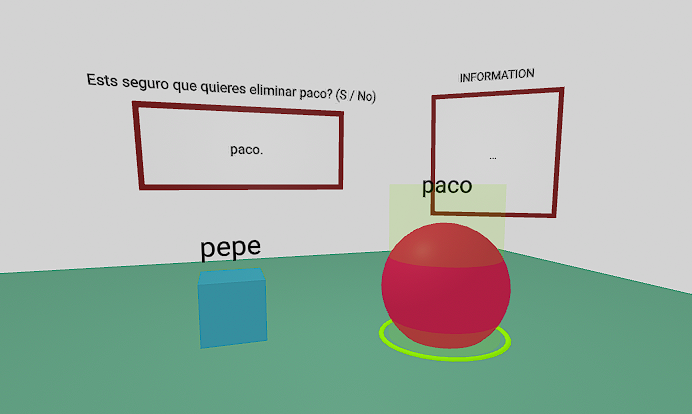
\includegraphics[width=0.6\linewidth]{img/generador_funcional_completo_eliminar.png}  % Ajusta el tamaño con width o height
    \caption{Funcionamiento de eliminar objetos con ID}  % Opcional: agrega una leyenda a la imagen
    \label{fig:eliminarObj}  % Opcional: añade una etiqueta para referenciar la imagen
  \end{figure} 

  \item \textbf{edit-mode-handler:} Este componente gestiona el modo de edición de objetos existentes en la escena, según el ID del objeto, como se ve en la Figura~\ref{fig:editarObj}.
  \begin{figure}[H]  % Puedes quitar la opción [H] si no necesitas que esté en esa posición exacta
    \centering
    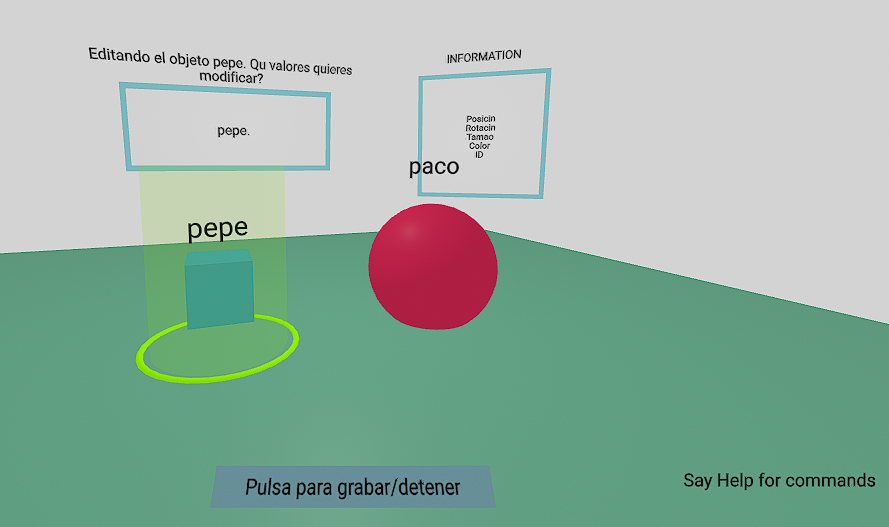
\includegraphics[width=0.6\linewidth]{img/generador_funcional_completo_editar.png}  % Ajusta el tamaño con width o height
    \caption{Funcionamiento de editar objetos con ID}  % Opcional: agrega una leyenda a la imagen
    \label{fig:editarObj}  % Opcional: añade una etiqueta para referenciar la imagen
  \end{figure} 


  \item \textbf{object-creator:} Este componente se encarga de instanciar los diferentes tipos de objetos en la escena basándose en los eventos recibidos, como se ve en la Figura~\ref{fig:generadorassets}.
  \begin{figure}[H]  % Puedes quitar la opción [H] si no necesitas que esté en esa posición exacta
    \centering
    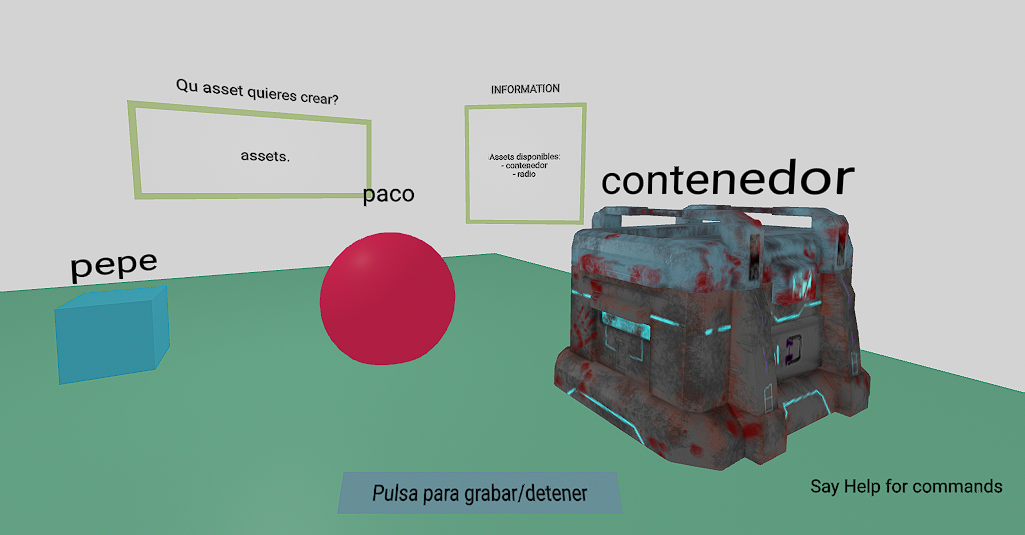
\includegraphics[width=0.6\linewidth]{img/generador_funcional_completo_assets.png}  % Ajusta el tamaño con width o height
    \caption{Funcionamiento del generador de assets}  % Opcional: agrega una leyenda a la imagen
    \label{fig:generadorassets}  % Opcional: añade una etiqueta para referenciar la imagen
  \end{figure} 
\end{itemize}

Además, se definen varias funciones utilitarias (\textbf{updateUserMessage, stepsPOS, stepsROT, stepCOLOR, stepID, stepSIZE, getEntityById, getLastCreatedEntity, createTorus}) para facilitar la manipulación de la escena y los objetos.

También se cambiaron y agregaron comandos nuevos al uso del \textbf{command-handler} así como \textbf{crear, editar, ayuda, salir}
Se añadieron paneles nuevos para añadir información extra que puede ser útil al usuario tanto escrita como visual, como se puede ver en los bordes de los paneles que cambian de color, dependiendo del estado en el que se encuentre la aplicación (verde=crear, rojo=eliminar \dots).
\subsection{Resultados}
\textbf{Gestión de nuevos comandos:} Integración de creación, edición y eliminación por voz mediante componentes dedicados (delete-object, edit-mode-handler, object-creator) y modificación avanzada con dynamic-modifier.

\textbf{Cambio en la estética y colocación de objetos:} Se modificó el HUD para hacerlo más agradable, visualmente y de ayuda para el usuario, creando así una escena sencilla.
\subsection{Lecciones aprendidas}

\textbf{Identificación de objetos:} Es crucial darle un nombre a los objetos para luego poder dar uso de las funciones de edición y eliminación específicas.

\textbf{Reutilización de código:} Las funciones utilitarias evitan la repetición.

\textbf{Retroalimentación al usuario:} Informar sobre los comandos y el estado es esencial.

\section{Sprint 5} 
\label{sec:sprint5}
La duración de este sprint fue de una semana. Durante este periodo se identificaron varios fallos críticos que llevaron a una reestructuración significativa del flujo de trabajo inicial.
\subsection{Objetivos}
\begin{itemize}
 
 \item Explorar la posibilidad de integración del proyecto con dispositivos VR/AR, específicamente las gafas Quest 3.
 \item Creación de servidor propio para peticiones de transcripción.
 
\end{itemize}
\subsection{Tareas Realizadas}

Durante este proceso se encontró el fallo más grande. En primer lugar, se quería realizar este proyecto íntegro en gafas VR/AR Quest3. 
Pero la API de reconocimiento de voz integrada en navegadores no fue soportada por el navegador de \textbf{Meta}, entonces se volvió a replantear todo lo trabajado con anterioridad.
Probamos con tecnologías diferentes de reconocimiento de voz, refactorizamos el componente que se encargaba de reconocimiento de voz dentro de nuestro proyecto de A-Frame.
Pero no se encontró ninguna solución, ya que no soportaba la detección del audio.

Por ello, se creó un servidor privado que fuese capaz de manejar los audios obtenidos del cliente y luego procesarlos y mandarlos a una API de \textbf{Speech-to-text} llamada Assembly AI, que devolverá la transcripción al servidor y este finalmente al cliente por medio del servidor.
Esta fue la parte desafiante del sprint. Ya se había manejado un servidor con anterioridad, pero este manejaba unos procesos simples y todo ocurría en el mismo ordenador, pero a la hora de conectarse otros dispositivos, dependía de permisos y certificaciones para hacer esta conexión posible.

La implementación de un servidor HTTPS funcional presentó un nuevo reto, ya que se necesitaba garantizar la conexión desde otros dispositivos dentro de la red local. Para ello, se abordaron los siguientes aspectos técnicos:

\textbf{-Certificado SSL:}SSL/server.key(clave privada) y SSL/server.crt(certificado público). En los navegadores aparecerá como “no seguro” si es autofirmado.

\textbf{-Configurar un servidor HTTPS} 

\textbf{-Acceso desde otros dispositivos en red local:}Ahora la conexión deberá hacerse al servidor, entonces en la URL deberemos apuntar a la IP del servidor que esté en la misma conexión de internet y con el puerto correspondiente(ej. https://<<IP>>:8080/)

\subsection{Resultados}
Tras la creación de certificados y configuraciones, se pudo conectar el servidor con las gafas de VR/AR Quest3. El problema era la detección del micrófono, que solo se hacía si el servidor tenía los permisos para HTTPS.

Como resultado, se consiguió la interacción completa esperada: el cliente envía el audio al servidor, este lo reenvía a Assembly AI para su transcripción, y finalmente el texto transcrito es devuelto al cliente para su visualización.

También hay que recalcar que para el uso de algunos complementos nos tocó usar una versión de A-Frame pasada, para poder usar el desplazamiento por la escena.
\subsection{Lecciones aprendidas}
\begin{itemize}
 \item Las limitaciones de plataformas específicas (como navegadores embebidos en dispositivos VR) pueden requerir rediseños profundos en la arquitectura del sistema.
 \item Contar con un servidor propio proporciona flexibilidad y control, pero también exige cumplir con requisitos de seguridad como HTTPS para trabajar con APIs modernas o acceder a funciones sensibles como el micrófono.
 \item La comunicación segura entre dispositivos en red local es posible incluso con certificados autofirmados, siempre y cuando se configuren correctamente.
\end{itemize}

\clearpage
\section{Sprint 6} 
\label{sec:sprint6}
Este Sprint duró 3 semanas, en donde se llevaron a cabo los últimos ajustes para la implementación final tanto en escritorio como para gafas VR/AR Quest3.
\subsection{Objetivos}
\begin{itemize}
 \item Mejora de la estética y colocación de objetos.
 \item Implementación de plugins extra para la visualización y decoraciones.
 \item Maquetado final de la demo para escritorio.
 \item Maquetado y unión del back-end y front-end para demo con gafas Quest3. 
\end{itemize}
\subsection{Tareas Realizadas}
Se mantuvo la posición de los objetos que dan información, además de agregar un plugin para que el panel completo siempre mirase a la cámara. Esto se realizó con un \texttt{\textbf{look-at}}.

Durante este sprint se decidió modificar un poco la visualización de los paneles y optamos por usar un plugin llamado \texttt{\textbf{html embed}} que permite incrustar HTML en los paneles de A-Frame, quedando de la forma que se ve en la Figura~\ref{fig:htmlembed}
  \begin{figure}[H]  % Puedes quitar la opción [H] si no necesitas que esté en esa posición exacta
    \centering
    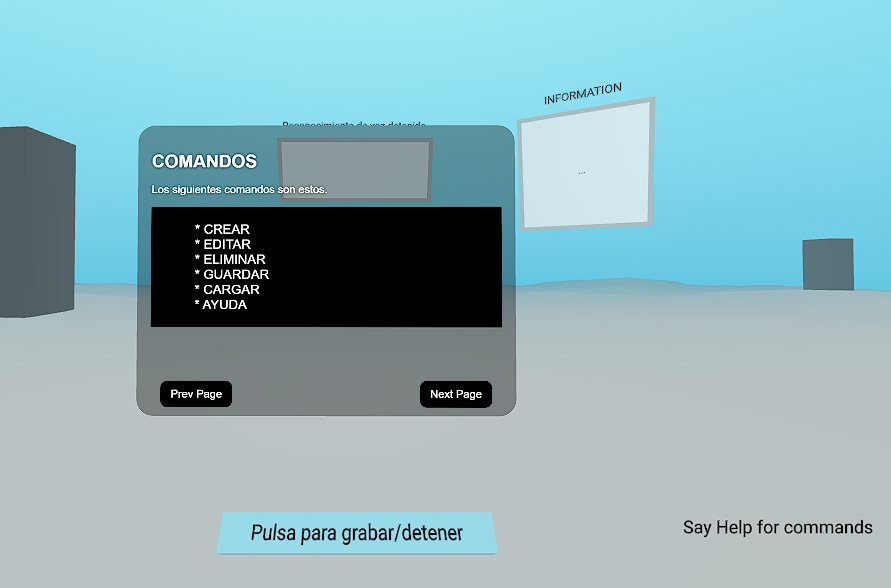
\includegraphics[width=0.4\linewidth]{img/htmlembed.png}  % Ajusta el tamaño con width o height
    \caption{Funcionamiento de htmlembed}  % Opcional: agrega una leyenda a la imagen
    \label{fig:htmlembed}  % Opcional: añade una etiqueta para referenciar la imagen
  \end{figure} 
Durante este sprint se añadieron también nuevos componentes al funcionamiento del proyecto, unos para la creación de objetos que llevasen otros componentes incrustados, de tal manera que con un solo componente se pudiese estructurar todo. 
Por otro lado, también se agregaron componentes para nuevos comandos tales como \textbf{Guardar} y \textbf{Cargar} escenas Figura~\ref{fig:componentes5}.
  \begin{figure}[H]  % Puedes quitar la opción [H] si no necesitas que esté en esa posición exacta
    \centering
    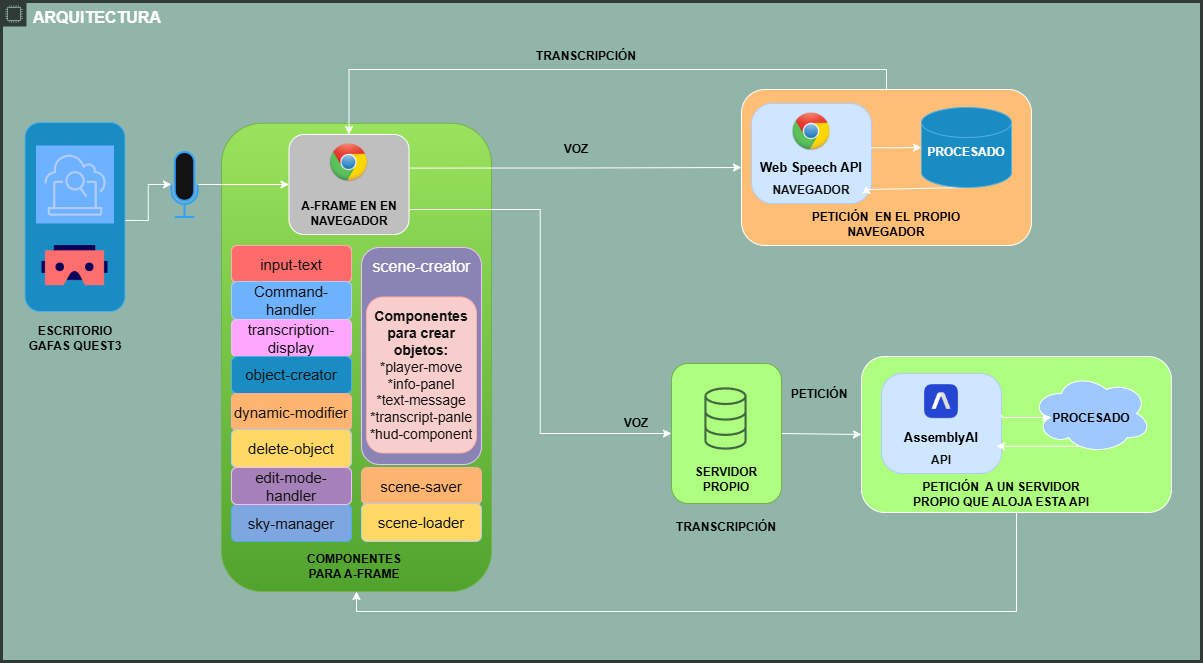
\includegraphics[width=0.6\linewidth]{img/componentes5.png}  % Ajusta el tamaño con width o height
    \caption{componentes finales agregados}  % Opcional: agrega una leyenda a la imagen
    \label{fig:componentes5}  % Opcional: añade una etiqueta para referenciar la imagen
  \end{figure} 
Finalmente, se hizo la inclusión de las demos para escritorio y gafas Quest3 en donde el cambio más significativo entre ellas es el componente \texttt{\textbf{'input-text'}}, el cual en la versión de escritorio usa \textbf{WebSpeechAPI} y en la versión de AR/VR usamos un servidor conectado a \textbf{AssemblyAI}.
\subsection{Resultados}

El desarrollo de componentes reutilizables mejoró la modularidad del sistema, permitiendo construir objetos más complejos con menos código y mayor coherencia visual.

También se logró una integración efectiva de entrada por voz, adaptada según la demo, lo que permitió mantener una experiencia coherente en ambos entornos.
\subsection{Lecciones aprendidas}
Una de las principales lecciones fue la importancia de diseñar con enfoque multiplataforma desde el inicio, considerando las capacidades y limitaciones propias de cada entorno. 

Adaptar interfaces y métodos de interacción según el dispositivo resultó crucial para garantizar una experiencia fluida y natural.

También se valoró el uso de herramientas externas y plugins, que ampliaron las posibilidades de diseño y funcionalidad sin comprometer el rendimiento.

Finalmente, se reafirmó la importancia de mantener una arquitectura limpia y desacoplada entre el front-end y el back-end, lo que facilitó la integración final de las demos.
\chapter{Resultados}
\label{chap:resultados}
\textbf{COMO SE USA AL USUARIO}: con capturas de pantalla\dots
\textbf{DESCRIPCION TECNICA PARA MANTENERLO A UN IGENIERO}
\begin{itemize}
  \item Que componentes que hay y como estan hechos
  \item como se relacionan los componentes
  \item que apis usan y como se utilizando
  \item el diagrama de uso..
  \item lo coge el component lo pasa a donde sea y lo devuelve\dots
\end{itemize}
\textbf{USO DE COMPONENTES PARA CONSTRUIR DISTINTAS APLICACIONES}
\begin{itemize}
  \item COMPONENTES QUE SIRVEN PARA X cosas
  \item SON reutilizables
  \item MODULAR Y COMO USARLA.
  \item COMO COMPONER LOS COMPONENTES.
\end{itemize}
\section{Flujo de funcionamiento} 
\label{sec:funcionamiento}
\begin{figure}[H]
  \centering
  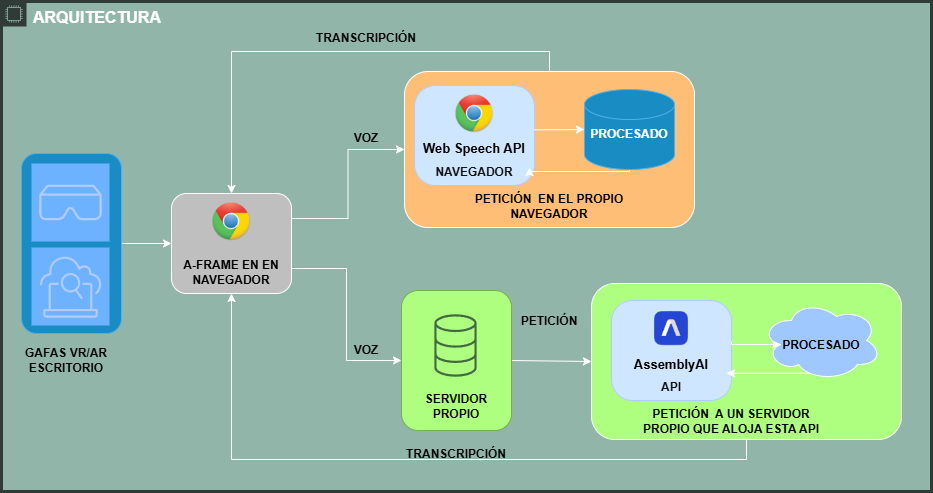
\includegraphics[width=14cm, keepaspectratio]{img/Arquitectura.png}
  \caption{Estructura del funcionamiento del Proyecto}
  \label{fig:arquitectura}
\end{figure}


El diagrama de la Figura~\ref{fig:arquitectura} muestra dos arquitecturas distintas para transcribir voz en una aplicación web VR/AR construida con A-Frame. En la primera demo, la transcripción se realiza directamente en el navegador usando la Web Speech API. Esto permite capturar la voz y procesarla sin necesidad de servidores externos, lo cual es rápido pero depende del soporte del navegador. En la segunda demo, la voz se envía a un servidor propio, que luego la reenvía a la API de AssemblyAI para su transcripción. Esta opción ofrece mayor precisión y capacidades avanzadas, aunque requiere una infraestructura adicional y puede tener más latencia.

se necesita el uso del 'NOMBRE DEL-.js' para el uso en html con la llamada a el scrpit y poner el componente en una entidad de la scena\dots
ademas de un componente que almacene los objetos llamado 'xxx'

** SEGUIR CON ESTO **

Descripción para usuario (manual de usuario)
Descripción de la implementación
\section{Componentes} 
\label{sec:Componentes}
\subsection{dynamic-modifier}
\begin{itemize}
  \item \textbf{stepsPOS(posKey, entity, transcript):} Permite modificar las coordenadas X, Y, Z de la posición en pasos. Al decir 'posición', se pregunta por la 'x', luego 'y', luego 'z'.
  \item \textbf{stepCOLOR(entity, transcript):} Intenta encontrar un color válido en el transcript utilizando un mapa (colorsMap) y actualiza el color del material del objeto.
  \item \textbf{stepID(entity, transcript):} Permite cambiar el id de la entidad y también actualiza el texto que se muestra sobre el objeto.
  \item \textbf{stepSIZE(entity, transcript):} Intenta extraer un número del transcript y lo aplica como un nuevo tamaño a todos los parámetros de la geometría del objeto (excepto primitive y otros parámetros específicos).
\end{itemize}

MEDICIONES DE TIEMPO PARA LAS RESPUESTAS, Y LOS CAMBIOS EN LA ESCENA \dots
\texttt{\textbf{command-handler:}} Es un componente que interpreta comandos de voz para crear objetos en la escena, pero con una entrada de audio configurable.
además de aplicar una reestructuración del código con el fin de mejorar la organización, escalabilidad y mantenibilidad del proyecto.
Depende de que otro componente en la escena realice el reconocimiento de voz y emita un evento transcription con el texto transcrito.
Durante su funcionamiento emite eventos a nivel de escena (\texttt{enter-create-mode, exit-create-mode}) para señalar el inicio y el fin del proceso de creación.
\texttt{\textbf{transcription-display:}} Tiene la función de mostrar en un elemento de texto 3D con un \textbf{ID} definido (\texttt{<a-text>}) la transcripción de voz proveniente de otro componente de la escena.
Se puede observar su uso en la Figura~\ref{fig:comandDemo4} en donde aparece los mensajes para el ususario en la parte superior de la caja de texto normal.

\texttt{\textbf{sky-manager:}} Se encarga de gestionar el color del fondo de la escena (<a-sky>) en respuesta a eventos personalizados emitidos a nivel de la escena provenientes del \texttt{\textbf{command-handler}}.

\begin{itemize}
  \item \textbf{delete-object:}Este componente maneja la lógica para eliminar objetos de la escena mediante comandos de voz.
  \begin{figure}[H]  % Puedes quitar la opción [H] si no necesitas que esté en esa posición exacta
    \centering
    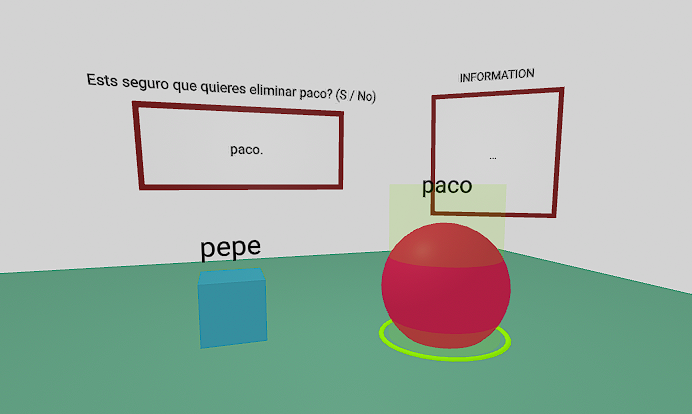
\includegraphics[width=0.8\linewidth]{img/generador_funcional_completo_eliminar.png}  % Ajusta el tamaño con width o height
    \caption{Funcionamiento de eliminar objetos con ID}  % Opcional: agrega una leyenda a la imagen
    \label{fig:eliminarObj}  % Opcional: añade una etiqueta para referenciar la imagen
  \end{figure} 
  Escucha el evento transcription.
  Pide al usuario el ID del objeto a eliminar. 
  Se visualiza un torus alrededor del objeto seleccionado para confirmar la eliminación.
  Permite confirmar o cancelar la eliminación mediante los comandos 'sí' o 'no'.
  Emite un mensaje de confirmación o cancelación al usuario.
  Permite salir del modo de eliminación con los comandos 'salir', 'atrás' o 'cambio'.

  \item \textbf{edit-mode-handler:} Este componente gestiona el modo de edición de objetos existentes en la escena.
  \begin{figure}[H]  % Puedes quitar la opción [H] si no necesitas que esté en esa posición exacta
    \centering
    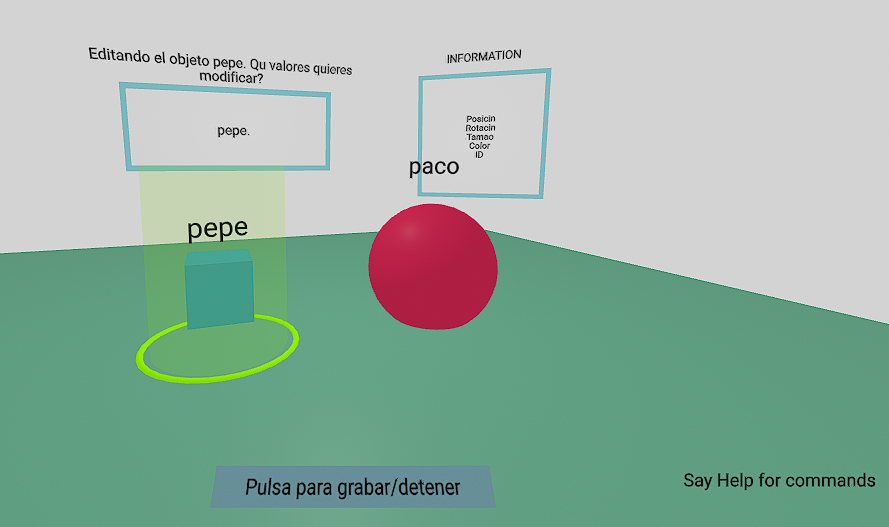
\includegraphics[width=0.8\linewidth]{img/generador_funcional_completo_editar.png}  % Ajusta el tamaño con width o height
    \caption{Funcionamiento de editar objetos con ID}  % Opcional: agrega una leyenda a la imagen
    \label{fig:editarObj}  % Opcional: añade una etiqueta para referenciar la imagen
  \end{figure} 
  Escucha el evento transcription.
  Pide al usuario el ID del objeto a editar.
  Busca el objeto por su ID y visualiza un torus alrededor para indicar que está en modo de edición.
  Utiliza la misma lógica de pasos y palabras clave que dynamic-modifier para permitir la modificación de las propiedades del objeto seleccionado.
  Elimina el torus al salir del modo de edición ("cambio").


  \item \textbf{object-creator:} Este componente se encarga de instanciar los diferentes tipos de objetos en la escena basándose en los eventos recibidos.
  \begin{figure}[H]  % Puedes quitar la opción [H] si no necesitas que esté en esa posición exacta
    \centering
    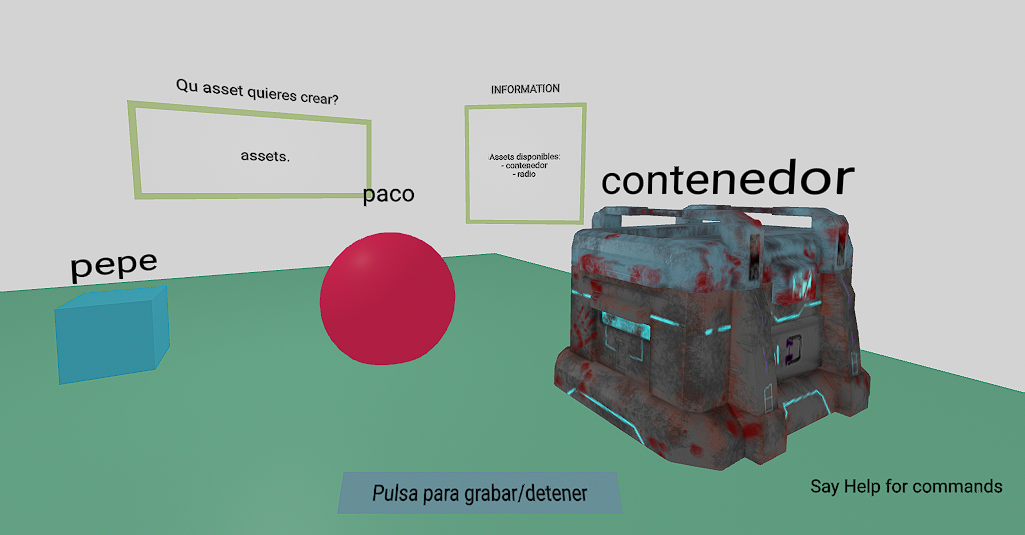
\includegraphics[width=0.8\linewidth]{img/generador_funcional_completo_assets.png}  % Ajusta el tamaño con width o height
    \caption{Funcionamiento del generador de assets}  % Opcional: agrega una leyenda a la imagen
    \label{fig:generadorassets}  % Opcional: añade una etiqueta para referenciar la imagen
  \end{figure} 
  Escucha el evento start-object-creation.
  Define los datos de creación para cada tipo de objeto (cubo, esfera, plano, luz, contenedor, radio) en formato JSON.
  Crea los elementos a-entity correspondientes con los atributos definidos (geometría, posición, material, etc.).
  Añade una clase 'dynamic-object' a los objetos creados.
  Crea una etiqueta de texto (aunque la función createText parece estar vacía en este fragmento).
  Establece las variables booleanas (modifyingBox, modifyingSphere, etc.) para indicar qué tipo de objeto se está modificando.

\end{itemize}
%%%%%%%%%%%%%%%%%%%%%%%%%%%%%%%%%%%%%%%%%%%%%%%EXPERIMENTACION Y VALIDACION%%%%%%%%%%%%%%%%%%%%%%%%%%%%%%%%%%%%%%
\chapter{Experimentos y validación}
\label{chap:experimentos}

Con el fin de validar la funcionalidad del sistema desarrollado 
\textbf{'una herramienta para la creación de objetos en entornos 3D mediante comandos de voz en A-Frame'} se realizó una serie de experimentos centrados en evaluar tanto el correcto reconocimiento de comandos como la experiencia de usuario.

Las pruebas se realizaron en un entorno controlado dentro de un habitacion que estaba equipada con una mesa de trabajo despejada, una silla ergonómica y la infraestructura tecnológica necesaria para ejecutar la aplicación.

Se utilizaron dos versiones del sistema para comparar el rendimiento entre plataformas, pero hay 3 posibilidades de uso:
\begin{itemize}
 \item Versión de escritorio con un monitor de 24 pulgadas
 \item Versión de móvil de gama media
 \item Versión en gafas Quest3 
\end{itemize}

Participaron cinco individuos con perfiles técnicos diversos, que no habian probado la aplicacion con anterioridad y ademas usuarios como el 1 y el 5 no habian experimentado el uso de gafas tipo Quest3. 
Esta variedad de perfiles se buscó intencionadamente para obtener una retroalimentación rica y representativa de diferentes niveles de familiaridad con la tecnología.


Las pruebas se llevaron a cabo utilizando la versión final de la demostración de la aplicación que estan alojadas en los siguientes repositorios.

\textbf{Versión de escritorio:} \url{https://github.com/R4CC00N/SpeechRecognition_in_Browser/tree/main/DemoEscritorio}

\textbf{Versión móvil:} \url{https://github.com/R4CC00N/SpeechRecognition_in_Browser/tree/main/DemoEscritorio}

\textbf{Versión en gafas Quest 3:} \url{https://github.com/R4CC00N/SpeechRecognition_in_Browser/tree/main/DemoVR}

Para cada una de las pruebas, un único experimentador guio a cada participante a través de la sesión, asegurándose de que las instrucciones se proporcionaran de manera estandarizada y consistente. 
Antes de comenzar cada tarea, el experimentador se dirigía al participante utilizando las siguientes palabras textuales:

``A continuación, te guiaré a través de una serie de tareas sencillas para evaluar cómo interactúas con el sistema. Por favor, sigue mis indicaciones y los mensajes informativos que aparecerán en la pantalla o dentro del entorno virtual.``

Una vez que el participante estaba preparado, el experimentador procedía a indicar cada tarea de forma secuencial, apoyándose también en los carteles de información integrados en la aplicación que proporcionaban recordatorios visuales de los comandos esperados. La secuencia de tareas que cada participante debía completar fue la siguiente:

\textbf{Creación de un cubo:} El experimentador indicaba verbalmente: ``Por favor, intenta crear un cubo utilizando el comando de voz \textbf{'crear'} y luego \textbf{'cubo'}.``
El participante debía accionar el sistema de reconocimiento de voz (pulsando el botón) y pronunciar el comando. Después de la acción del usuario, se observaba si el cubo se creaba correctamente en la escena y avisara al experimentador.

\textbf{Cambio de color del objeto:} Una vez creado el cubo, el experimentador dirá: ``Ahora, por favor, intenta cambiar el color del cubo a rojo utilizando el comando \textbf{'color'} y acto seguido \textbf{'rojo'}.`` 
El participante debía activar el reconocimiento de voz si se desactivo previamente y pronunciar el comando. En el momento en el que el color del cubo cambiaba a rojo según lo esperado se avisaba al experimentador.

\textbf{Posicionamiento del objeto:} Tras el cambio de color, el experimentador instruía: ``Ahora, intenta mover el cubo a otra ubicación dentro de la escena. Puedes usar el comando \textbf{'posicion'} y seguir las instrucciones en la información de la aplicación para especificar coordenadas." Se observaba si el participante lograba desplazar el objeto utilizando los comandos de movimiento disponibles y una vez conseguido se avisaba al experimentador.

\textbf{Eliminación del objeto:} Finalmente, el experimentador pedía: ``Por favor, elimina el cubo de la escena utilizando el comando \textbf{'eliminar'}.`` Se verificaba si el objeto desaparecía de la escena tras la ejecución del comando por parte del usuario.

\textbf{Manejo libre de la aplicación:} Después de completar las tareas guiadas, el experimentador indicaba: ``Ahora tienes unos minutos para explorar libremente la aplicación. Intenta crear otros objetos, cambiar sus propiedades o realizar cualquier acción que te parezca interesante utilizando los comandos de voz que recuerdes o que veas en la información.`` 
Durante este tiempo, se observaba cómo el participante interactuaba con el sistema sin indicaciones directas, los comandos que intentaba utilizar y cualquier dificultad que pudiera encontrar.



\section{Diseño Experimental}
El experimento se enfocó en medir tres aspectos principales del sistema:

\textbf{Objetivos}
\begin{itemize}
 \item Precisión del reconocimiento de voz.
 \item Facilidad de uso e intuición de los comandos.
 \item Tiempo medio desde la grabación de voz hasta la creación de objetos.
 \item Conseguir realimentacion de los usuarios sobre la experiencia.
\end{itemize}
\section{Resultados}
De 20 comandos de reconocimiento de voz se han obtenido los siguientes resultados en cada versión, añadiendo las observaciones más destacadas de cada una en el Cuadro~\ref{tab:precision_comandos}
\subsection{Precisión del Reconocimiento de Voz}

\begin{table}[H]
\centering
\begin{tabular}{|l|c|c|p{6cm}|}
\hline
\textbf{Usuario} & \textbf{Plataforma} & \textbf{Comandos exitosos} & \textbf{Observaciones} \\
\hline
Usuario 1 & Quest3 & 19 & Reconocimiento lento, modalidad de grabación de audio molesta. \\
\hline
Usuario 2 & Escritorio  & 18 & Reconocimiento rapido, errores con las transcripciones en algunos casos. \\
\hline
Usuario 3 & Móvil & 17 & Problemas con la interfaz para grabar audio, una vez obtenido el manejo, bastante fluido gracias a los mensajes de información \\
\hline
Usuario 4 & Escritorio  & 17 & Sin demoras en respuesta, no tiene comandos encadenados \\
\hline
Usuario 5 & Quest3 & 18 & Alta precisión en acento marcado, ligeras demoras en respuesta. \\
\hline
\end{tabular}
\caption{Porcentaje de reconocimiento de comandos por usuario y plataforma}
\label{tab:precision_comandos}
\end{table}


\subsection{Tiempo Promedio por Tarea}
\begin{table}[H]
\centering
\begin{tabular}{|l|c|c|c|p{6cm}|}
\hline
\textbf{Usuario} & \textbf{Crear objeto} & \textbf{Cambiar color} & \textbf{Mover objeto} & \textbf{Eliminar objeto} \\
\hline
Usuario 1 & Quest3 & 95\% & Reconocimiento lento, modalidad de grabación de audio molesta. \\
\hline
Usuario 2 & Escritorio  & 90\% & Reconocimiento rapido, errores con las transcripciones en algunos casos. \\
\hline
Usuario 3 & Móvil & 85\% & Problemas con la interfaz para grabar audio, una vez obtenido el manejo, bastante fluido gracias a los mensajes de información \\
\hline
Usuario 4 & Escritorio  & 85\% & Sin demoras en respuesta, no tiene comandos encadenados \\
\hline
Usuario 5 & Quest3 & 90\% & Alta precisión en acento marcado, ligeras demoras en respuesta. \\
\hline
\end{tabular}
\caption{Porcentaje de reconocimiento de comandos por usuario y plataforma}
\label{tab:precision_comandos}
\end{table}
\begin{itemize}
 \item \textbf{Crear objeto:} 3–5 segundos.
 \item \textbf{Cambiar color:} 2–3 segundos.
 \item \textbf{Mover objeto:} 4–6 segundos.
 \item \textbf{Eliminar objeto:} 2 segundos promedio.
\end{itemize}

Se observó que los tiempos en la versión Quest3 fueron ligeramente más altos debido al retardo en la conexión al servidor externo.

\subsection{Opiniones de los Usuarios}

Las opiniones recogidas al final de las pruebas fueron mayoritariamente positivas. A continuación se resumen algunos comentarios:

\begin{itemize}
 \item \textbf{Usuario 1:} "La experiencia en realidad virtual es muy inmersiva. Me gustaría poder usar frases más naturales y mejorar el tiempo de espera. Además, el manejo de grabar y parar de grabar por cada comando me pareció molesto."
 \item \textbf{Usuario 2:} "Sorprendido por la precisión del reconocimiento. Muy útil para crear escenas rápidamente y además muy vistosas."
 \item \textbf{Usuario 5:} "Solo bastan unos minutos para entender cómo manejar la aplicación, la parte de ejecución libre fue la mejor."
\end{itemize}

\section{Conclusión de Validación}

Los resultados obtenidos muestran que el proyecto cumple con los objetivos planteados: permite la creación y manipulación de objetos 3D mediante comandos de voz de forma eficiente y accesible, en entornos de escritorio y VR. La precisión en el reconocimiento fue alta en ambos entornos, y los usuarios consideraron la experiencia intuitiva y útil.

Es cierto que aún existen limitaciones como manejo de envío de audios para las transcripciones y latencia alta en una versión del proyecto.


\cleardoublepage

%%%%%%%%%%%%%%%%%%%%%%%%%%%%%%%%%%%%%%%%%%%%%%%%%%%%%%%%%%%%%%%%%%%%%%%%%%%%%%%%
%%%%%%%%%%%%%%%%%%%%%%%%%%%%%%%%%%%%%%%%%%%%%%%%%%%%%%%%%%%%%%%%%%%%%%%%%%%%%%%%
% CONCLUSIONES %
%%%%%%%%%%%%%%%%%%%%%%%%%%%%%%%%%%%%%%%%%%%%%%%%%%%%%%%%%%%%%%%%%%%%%%%%%%%%%%%%

\cleardoublepage
\chapter{Conclusiones}
\label{chap:conclusiones}


\section{Consecución de objetivos}
\label{sec:consecucion-objetivos}

DEBEMOS REVISAR SI LOS OBJETIVOS PLANTEADOS ESTAN BIEN PARA SEGUIR POR AQUI.

\section{Esfuerzo y recursos dedicados}
\label{sec:esfuerzo-recursos}

Se ha dividido el proyecto por sprint y se ha hablado en cada sprint de su duracion en semanas, pero aun no destaca el tiempo que se le ha dedicado.

Durante el primer sprint \textbf{Investigación y Prototipado Inicial}, la parte mas larga a mi parecer fue leer documentacion y buscar informacion de diferentes tecnologias de reconocimiento de voz,
\begin{itemize}
  \item La primera semana se busco informacion cada dia en torno a 2 horas excepto los fines de semana.
  \item La segunda semana se realizaron diferentes experimentos de cual seria la posible implementacion para la deteccion de voz y cual se elegiria para ello fue en torno a 3 horas durante viernes a domingo. 
  \item La tercera semana se realizo una incrustacion del reconocimiento de voz y A-Frame en la que se trabajo durante 2 horas diarias de lunes a miercoles.
\end{itemize}
Dandonos un tiempo de trabajo en el primer sprint de 31 horas.

Para el segundo sprint \textbf{Desarrollo de A-FRAME Base}, la parte mas compleja fue el manejo y creación de componentes para crear objetos primitivos.
\begin{itemize}
  \item La primera semana para la creación de objetos primitivos se trabajo durante 2 horas diarias durante 5 dias a la semana.
  \item La segunda semana se reestructuro el codigo y se creo manejadores para el componente de cracion de objetos este sprint se trabajo 4 horas solo sabado y domingo.
\end{itemize}
Dandonos un tiempo de trabajo en el segundo sprint de 18 horas.

Para el tercer sprint \textbf{Funcionalidades y Componentes}, la parte mas larga fue la creacion de componentes nuevos por el hecho de que se debian tener conexion entre componentes para que funcionasen.
\begin{itemize}
  \item La primera semana para el aumento de comandos se trabajo por 3 horas miercoles, jueves y viernes.
  \item La segunda semana para la creacion de escena simple, solucion de problemas y funciones para componentes se trabajo 3 horas durante viernes a lunes.
\end{itemize}
Dandonos un tiempo de trabajo en el tercer sprint de 21 horas.

Para el cuarto sprint \textbf{Mejora de componentes y Mejora Visual}.
\begin{itemize}
  \item La primera semana para creacion de componentes extra y modificacion de escena se trabajo 3 horas solo sabado y domingo.
  \item La segunda semana para crear comandos nuevos se trabajo 2 horas diarias durante la semana.
\end{itemize}
Dandonos un tiempo de trabajo en el cuarto sprint de 16 horas.

Para el quito sprint \textbf{integración en VR/AR}.
\begin{itemize}
  \item La semana para crear el server y hacer pruebas en las gafas topmo entorno a 6 horas de un solo dia.
\end{itemize}

Para el sexto sprint \textbf{Pasos finales}.
\begin{itemize}
  \item La primera semana para nuevos componentes se trabajo en ella durante 2 horas diarias toda la semana.
  \item La segunda semana en la implementacion de plugins y pruebas se trabajo entorno a 4 horas diarias durante el finde semana
  \item La tercera semana en la maquetacion y union de las demos se trabajo en torno a 3 horas diarias durante la semana.
\end{itemize}
Dandonos un tiempo de trabajo en el cuarto sprint de 36 horas.

Cabe recalcar que el proyecto se empezo a inicios de diciembre y se ha ido compaginando con el trabajo y las semanas de vacaciones, por ello es que se ha trabajado en la parte del codigo durante 4 meses aproximadamente y 1 mes mas en la parte de la memoria

\textbf{Diagrama de Gantt - Sprints}

\begin{ganttchart}[
  hgrid,
  vgrid,
  title label font=\bfseries,
  bar label font=\small,
  bar/.style={fill=blue!50}
]{1}{18}
 \gantttitle{Semanas}{18} \\
 \gantttitlelist{1,...,18}{1} \\
 \ganttbar{Investigación y Prototipado}{1}{3} \\
 \ganttbar{Desarrollo base}{4}{5} \\
 \ganttbar{Funcionalidades y Componentes}{6}{7} \\
 \ganttbar{Componentes extras}{8}{9} \\
 \ganttbar{Integración Quest3}{10}{10} \\
 \ganttbar{Demo y unión final}{11}{13} 
 \ganttbar{}{15}{15}\\
 \ganttbar{Memoria}{15}{18} \\ 
\end{ganttchart}

\subsection{Planificación temporal}
\label{sec:planificacion-temporal}

Con el diagrama de GANTT sirve?¿

\section{Aplicación de lo aprendido}
\label{sec:aplicacion}

...EN COSNTRUCCIÓN AÚN...

\section{Lecciones aprendidas}
\label{sec:lecciones_aprendidas}
A lo largo del desarollo de este proyecto, se ha adquirido un conocimiento variado y profundo en tecnologias involucradas en la creacion de la aplicacion.
\begin{itemize}
  \item Se ha profundizado en el uso de A-Frame principalmente, necesario para la creacion de experiencias en realidad virtual.
  \item Se indago profundamente en la construccion de componentes para A-Frame, con diferentes funcionalidades.
  \item Se profundizo en diferentes programas de deteccion de voz y sus aplicaciones.
  \item Creacion de un servidor privado para conexiones mediante HTTPS.
  \item Trabajar con dispositivos de VR/AR como las Quest3.
  \item Se mejoro el manejo de JavaScript, aunque aplicado a el entorno de A-Frame.
  \item Se ha aprendido a utilizar LaTex para la realizacion de documentos de investigacion y tecnicos como es la memoria.
\end{itemize}


\section{Trabajos futuros}
\label{sec:trabajos_futuros}

En este apartado se van a mencionar posibles mejoras e ideas que se pueden implementar para mejorar esta aplicacion:
\begin{itemize}
  \item Se pueden mejorar la deteccion de comandos encadenados, de tal manera que si detectase en una frase todos los atributos necesarios no haria falta la respuesta del componente para pedir cada dato.
  Esto ayudaria al dinamismo para creacion de escenas, ademas de evitar tiempos de espera entre comandos.
  \item Se pueden añadir comando para poder editar todos los parametros de cada objeto primitivo en la libreria de A-Frame. Por si es necesario la super edicion de objetos.
  \item Se podria integrar un modelo de lenguaje para que el programa entienda diminutivos, sinonimos, etc.
  \item En el tema visual, se podria añadir una interfaz que muestre al usuario que propiedades puede modificar dentro de una entidad, de esta manera ayudaria a saber como acceder y que valores se pueden dar.
  \item Tambien en el tema de retroalimentacion del programa al usuario, se podria añadir una funcion de voz (text-to-speech) para que devuelva los mensajes que ahora son de ayuda en texto, mediante la voz.
  \item Finalmente se podria crear un juego de plataformas simple en donde la dinamica principal para pasar el mapa sea la creacion de objetos con colisiones mediante comandos de voz e incluso crear objetos por voz para poder enfrentar enemigos, esta idea de juego aprovecharia al maximo la creacion de objetos y trancripcion de comandos de tal manera que la experiencia de juego se veria enriquecida.
\end{itemize}
\cleardoublepage
\appendix
\chapter{Manual de usuario}
\label{app:manual}

Esto es un apéndice.
Si has creado una aplicación, siempre viene bien tener un manual de usuario.
Pues ponlo aquí.

%%%%%%%%%%%%%%%%%%%%%%%%%%%%%%%%%%%%%%%%%%%%%%%%%%%%%%%%%%%%%%%%%%%%%%%%%%%%%%%%
%%%%%%%%%%%%%%%%%%%%%%%%%%%%%%%%%%%%%%%%%%%%%%%%%%%%%%%%%%%%%%%%%%%%%%%%%%%%%%%%
% BIBLIOGRAFIA %
%%%%%%%%%%%%%%%%%%%%%%%%%%%%%%%%%%%%%%%%%%%%%%%%%%%%%%%%%%%%%%%%%%%%%%%%%%%%%%%%

\cleardoublepage

% Las siguientes dos instrucciones es todo lo que necesitas
% para incluir las citas en la memoria
\bibliographystyle{abbrv}
\bibliography{memoria}  % memoria.bib es el nombre del fichero que contiene
% las referencias bibliográficas. Abre ese fichero y mira el formato que tiene,
% que se conoce como BibTeX. Hay muchos sitios que exportan referencias en
% formato BibTeX. Prueba a buscar en http://scholar.google.com por referencias
% y verás que lo puedes hacer de manera sencilla.
% Más información: 
% http://texblog.org/2014/04/22/using-google-scholar-to-download-bibtex-citations/

\end{document}
